% Options for packages loaded elsewhere
% Options for packages loaded elsewhere
\PassOptionsToPackage{unicode}{hyperref}
\PassOptionsToPackage{hyphens}{url}
\PassOptionsToPackage{dvipsnames,svgnames,x11names}{xcolor}
%
\documentclass[
  spanish,
  11pt,
  a4paper,
  DIV=11,
  numbers=noendperiod]{scrartcl}
\usepackage{xcolor}
\usepackage[top=24mm,bottom=24mm,left=24mm,right=24mm,headheight=14pt,headsep=8mm]{geometry}
\usepackage{amsmath,amssymb}
\setcounter{secnumdepth}{5}
\usepackage{iftex}
\ifPDFTeX
  \usepackage[T1]{fontenc}
  \usepackage[utf8]{inputenc}
  \usepackage{textcomp} % provide euro and other symbols
\else % if luatex or xetex
  \usepackage{unicode-math} % this also loads fontspec
  \defaultfontfeatures{Scale=MatchLowercase}
  \defaultfontfeatures[\rmfamily]{Ligatures=TeX,Scale=1}
\fi
\usepackage{lmodern}
\ifPDFTeX\else
  % xetex/luatex font selection
\fi
% Use upquote if available, for straight quotes in verbatim environments
\IfFileExists{upquote.sty}{\usepackage{upquote}}{}
\IfFileExists{microtype.sty}{% use microtype if available
  \usepackage[]{microtype}
  \UseMicrotypeSet[protrusion]{basicmath} % disable protrusion for tt fonts
}{}
\makeatletter
\@ifundefined{KOMAClassName}{% if non-KOMA class
  \IfFileExists{parskip.sty}{%
    \usepackage{parskip}
  }{% else
    \setlength{\parindent}{0pt}
    \setlength{\parskip}{6pt plus 2pt minus 1pt}}
}{% if KOMA class
  \KOMAoptions{parskip=half}}
\makeatother
% Make \paragraph and \subparagraph free-standing
\makeatletter
\ifx\paragraph\undefined\else
  \let\oldparagraph\paragraph
  \renewcommand{\paragraph}{
    \@ifstar
      \xxxParagraphStar
      \xxxParagraphNoStar
  }
  \newcommand{\xxxParagraphStar}[1]{\oldparagraph*{#1}\mbox{}}
  \newcommand{\xxxParagraphNoStar}[1]{\oldparagraph{#1}\mbox{}}
\fi
\ifx\subparagraph\undefined\else
  \let\oldsubparagraph\subparagraph
  \renewcommand{\subparagraph}{
    \@ifstar
      \xxxSubParagraphStar
      \xxxSubParagraphNoStar
  }
  \newcommand{\xxxSubParagraphStar}[1]{\oldsubparagraph*{#1}\mbox{}}
  \newcommand{\xxxSubParagraphNoStar}[1]{\oldsubparagraph{#1}\mbox{}}
\fi
\makeatother


\usepackage{longtable,booktabs,array}
\usepackage{calc} % for calculating minipage widths
% Correct order of tables after \paragraph or \subparagraph
\usepackage{etoolbox}
\makeatletter
\patchcmd\longtable{\par}{\if@noskipsec\mbox{}\fi\par}{}{}
\makeatother
% Allow footnotes in longtable head/foot
\IfFileExists{footnotehyper.sty}{\usepackage{footnotehyper}}{\usepackage{footnote}}
\makesavenoteenv{longtable}
\usepackage{graphicx}
\makeatletter
\def\fps@figure{htbp}
\makeatother



\ifLuaTeX
\usepackage[bidi=basic]{babel}
\else
\usepackage[bidi=default]{babel}
\fi
% get rid of language-specific shorthands (see #6817):
\let\LanguageShortHands\languageshorthands
\def\languageshorthands#1{}


\setlength{\emergencystretch}{3em} % prevent overfull lines

\providecommand{\tightlist}{%
  \setlength{\itemsep}{0pt}\setlength{\parskip}{0pt}}



 


\newcommand{\practicaPdfCoverImage}{../resources/practica9/images/house_100mm.png}
% PDF style for Practica 9.
% A modest university handout look: classical type, clear hierarchy,
% restrained color, and durable code/callout styling.

\usepackage{graphicx}
\usepackage[export]{adjustbox}
\usepackage{fontspec}
\usepackage{microtype}
\usepackage{scrlayer-scrpage}
\usepackage{tikz}
\usepackage{fvextra}
\usepackage{caption}
\usepackage{subcaption}
\usepackage[skins,breakable]{tcolorbox}

\providecommand{\practicaPdfCoverImage}{}

\definecolor{uzaInk}{HTML}{172033}
\definecolor{uzaMuted}{HTML}{5F6B7A}
\definecolor{uzaBlue}{HTML}{1F5F8B}
\definecolor{uzaBlueDark}{HTML}{153E5C}
\definecolor{uzaCyan}{HTML}{EAF4F7}
\definecolor{uzaLine}{HTML}{D7E2EA}
\definecolor{uzaCodeBg}{HTML}{F5F7F9}
\definecolor{uzaTip}{HTML}{237A57}
\definecolor{uzaWarn}{HTML}{A65F00}

\IfFontExistsTF{TeX Gyre Pagella}{
  \setmainfont{TeX Gyre Pagella}
}{}
\IfFontExistsTF{TeX Gyre Heros}{
  \setsansfont{TeX Gyre Heros}
}{}
\IfFontExistsTF{TeX Gyre Cursor}{
  \setmonofont{TeX Gyre Cursor}[Scale=0.86]
}{
  \setmonofont{Latin Modern Mono}[Scale=0.88]
}

\KOMAoptions{parskip=half}
\setlength{\parindent}{0pt}
\setlength{\parskip}{0.55em plus 0.15em minus 0.08em}
\linespread{1.035}

\addtokomafont{disposition}{\sffamily\color{uzaBlueDark}}
\addtokomafont{section}{\LARGE}
\addtokomafont{subsection}{\Large}
\addtokomafont{subsubsection}{\normalsize\bfseries}
\RedeclareSectionCommand[beforeskip=2.2em plus 0.4em minus 0.2em,afterskip=1.0em]{section}
\RedeclareSectionCommand[beforeskip=1.2em,afterskip=0.55em]{subsection}
\RedeclareSectionCommand[beforeskip=1.0em,afterskip=0.35em]{subsubsection}

\clearpairofpagestyles
\automark[section]{section}
\ihead{\sffamily\footnotesize\textcolor{uzaMuted}{Informática (30717)}}
\ohead{\sffamily\footnotesize\textcolor{uzaMuted}{\headmark}}
\cfoot{\sffamily\small\textcolor{uzaMuted}{\pagemark}}
\setkomafont{pageheadfoot}{\normalfont}
\KOMAoptions{headsepline=0.35pt}
\addtokomafont{headsepline}{\color{uzaLine}}

\makeatletter
\AtBeginDocument{%
  \hypersetup{
    linkcolor=uzaBlueDark,
    urlcolor=uzaBlue,
    citecolor=uzaBlueDark
  }%
  \@ifundefined{Highlighting}{%
    \DefineVerbatimEnvironment{Highlighting}{Verbatim}{
      commandchars=\\\{\},
      fontsize=\small,
      breaklines=true,
      breakanywhere=true
    }%
  }{%
    \RecustomVerbatimEnvironment{Highlighting}{Verbatim}{
      commandchars=\\\{\},
      fontsize=\small,
      breaklines=true,
      breakanywhere=true
    }%
  }%
  \@ifundefined{Shaded}{%
    \newenvironment{Shaded}{%
      \begin{tcolorbox}[
        enhanced,
        breakable,
        sharp corners,
        boxrule=0.25pt,
        colback=uzaCodeBg,
        colframe=uzaLine,
        borderline west={1.4pt}{0pt}{uzaBlue},
        left=2mm,
        right=2mm,
        top=1.4mm,
        bottom=1.4mm,
        before skip=0.75em,
        after skip=0.75em
      ]%
    }{%
      \end{tcolorbox}%
    }%
  }{%
    \renewenvironment{Shaded}{%
      \begin{tcolorbox}[
        enhanced,
        breakable,
        sharp corners,
        boxrule=0.25pt,
        colback=uzaCodeBg,
        colframe=uzaLine,
        borderline west={1.4pt}{0pt}{uzaBlue},
        left=2mm,
        right=2mm,
        top=1.4mm,
        bottom=1.4mm,
        before skip=0.75em,
        after skip=0.75em
      ]%
    }{%
      \end{tcolorbox}%
    }%
  }%
}
\makeatother

\newcommand{\PracticeCode}[1]{%
  \begin{Shaded}%
  \VerbatimInput[
    fontsize=\small,
    breaklines=true,
    breakanywhere=true
  ]{#1}%
  \end{Shaded}%
}

\makeatletter
\renewcommand{\maketitle}{%
  \begin{titlepage}
    \thispagestyle{empty}
    \begin{tikzpicture}[remember picture,overlay]
      \fill[uzaCyan] (current page.north west) rectangle ([yshift=-72mm]current page.north east);
      \fill[uzaBlue] (current page.north west) rectangle ([xshift=7mm]current page.south west);
    \end{tikzpicture}
    \vspace*{12mm}
    {\sffamily\small\bfseries\textcolor{uzaBlue}{INFORMÁTICA (30717)}}\par
    \vspace{5mm}
    {\sffamily\bfseries\fontsize{30}{35}\selectfont\textcolor{uzaInk}{\@title}}\par
    \vspace{3mm}
    {\sffamily\Large\textcolor{uzaMuted}{Grado en Estudios en Arquitectura}}\par
    \vspace{8mm}
    {\color{uzaBlue}\rule{\textwidth}{0.6pt}}\par
    \if\relax\detokenize\expandafter{\practicaPdfCoverImage}\relax
    \else
      \vspace{5mm}
      {\centering\includegraphics[width=\textwidth,height=78mm,keepaspectratio]{\practicaPdfCoverImage}\par}
    \fi
    \vfill
    {\sffamily\large\textcolor{uzaBlueDark}{Universidad de Zaragoza}}\par
    \vspace{2mm}
    {\sffamily\small\textcolor{uzaMuted}{Material de prácticas del curso 2025--2026}}\par
  \end{titlepage}
}
\makeatother

\captionsetup{
  font={small,sf},
  labelfont={bf,color=uzaBlueDark},
  textfont={color=uzaInk},
  justification=centering,
  singlelinecheck=false,
  skip=6pt
}
\captionsetup[subfigure]{
  font={small,sf},
  labelfont={bf,color=uzaBlueDark},
  justification=centering,
  singlelinecheck=true,
  skip=4pt
}

\newcommand{\PracticeCredit}[1]{\textcolor{uzaMuted}{#1}}
\newcommand{\PracticeImagePair}[6]{%
  \begin{figure}[tbp]
    \centering
    \begin{minipage}[t]{0.485\linewidth}
      \includegraphics[width=\linewidth]{#3}
      \vspace{2mm}
      \centering{\sffamily\footnotesize #4}
    \end{minipage}\hfill
    \begin{minipage}[t]{0.485\linewidth}
      \includegraphics[width=\linewidth]{#5}
      \vspace{2mm}
      \centering{\sffamily\footnotesize #6}
    \end{minipage}
    \caption{\label{#1}#2}
  \end{figure}
}

\renewcommand{\arraystretch}{1.16}
\setlength{\tabcolsep}{6pt}
\setkeys{Gin}{center}

% Quarto callout colors are referenced by generated tcolorbox options.
% Apply them at document start so they win over Quarto's defaults.
\AtBeginDocument{%
  \definecolor{quarto-callout-note-color}{HTML}{1F5F8B}%
  \definecolor{quarto-callout-note-color-frame}{HTML}{1F5F8B}%
  \definecolor{quarto-callout-tip-color}{HTML}{237A57}%
  \definecolor{quarto-callout-tip-color-frame}{HTML}{237A57}%
  \definecolor{quarto-callout-warning-color}{HTML}{A65F00}%
  \definecolor{quarto-callout-warning-color-frame}{HTML}{A65F00}%
  \definecolor{quarto-callout-important-color}{HTML}{9B2C2C}%
  \definecolor{quarto-callout-important-color-frame}{HTML}{9B2C2C}%
  \definecolor{quarto-callout-caution-color}{HTML}{B45309}%
  \definecolor{quarto-callout-caution-color-frame}{HTML}{B45309}%
}

\KOMAoption{captions}{tableheading}
\makeatletter
\@ifpackageloaded{tcolorbox}{}{\usepackage[skins,breakable]{tcolorbox}}
\@ifpackageloaded{fontawesome5}{}{\usepackage{fontawesome5}}
\definecolor{quarto-callout-color}{HTML}{909090}
\definecolor{quarto-callout-note-color}{HTML}{0758E5}
\definecolor{quarto-callout-important-color}{HTML}{CC1914}
\definecolor{quarto-callout-warning-color}{HTML}{EB9113}
\definecolor{quarto-callout-tip-color}{HTML}{00A047}
\definecolor{quarto-callout-caution-color}{HTML}{FC5300}
\definecolor{quarto-callout-color-frame}{HTML}{acacac}
\definecolor{quarto-callout-note-color-frame}{HTML}{4582ec}
\definecolor{quarto-callout-important-color-frame}{HTML}{d9534f}
\definecolor{quarto-callout-warning-color-frame}{HTML}{f0ad4e}
\definecolor{quarto-callout-tip-color-frame}{HTML}{02b875}
\definecolor{quarto-callout-caution-color-frame}{HTML}{fd7e14}
\makeatother
\makeatletter
\@ifpackageloaded{caption}{}{\usepackage{caption}}
\AtBeginDocument{%
\ifdefined\contentsname
  \renewcommand*\contentsname{Tabla de contenidos}
\else
  \newcommand\contentsname{Tabla de contenidos}
\fi
\ifdefined\listfigurename
  \renewcommand*\listfigurename{Listado de Figuras}
\else
  \newcommand\listfigurename{Listado de Figuras}
\fi
\ifdefined\listtablename
  \renewcommand*\listtablename{Listado de Tablas}
\else
  \newcommand\listtablename{Listado de Tablas}
\fi
\ifdefined\figurename
  \renewcommand*\figurename{Figura}
\else
  \newcommand\figurename{Figura}
\fi
\ifdefined\tablename
  \renewcommand*\tablename{Tabla}
\else
  \newcommand\tablename{Tabla}
\fi
}
\@ifpackageloaded{float}{}{\usepackage{float}}
\floatstyle{ruled}
\@ifundefined{c@chapter}{\newfloat{codelisting}{h}{lop}}{\newfloat{codelisting}{h}{lop}[chapter]}
\floatname{codelisting}{Listado}
\newcommand*\listoflistings{\listof{codelisting}{Listado de Listados}}
\makeatother
\makeatletter
\makeatother
\makeatletter
\@ifpackageloaded{caption}{}{\usepackage{caption}}
\@ifpackageloaded{subcaption}{}{\usepackage{subcaption}}
\makeatother
\usepackage{bookmark}
\IfFileExists{xurl.sty}{\usepackage{xurl}}{} % add URL line breaks if available
\urlstyle{same}
\hypersetup{
  pdftitle={Práctica 9: Visualizador 3D},
  pdflang={es},
  colorlinks=true,
  linkcolor={blue},
  filecolor={Maroon},
  citecolor={Blue},
  urlcolor={Blue},
  pdfcreator={LaTeX via pandoc}}


\title{Práctica 9: Visualizador 3D}
\author{}
\date{}
\begin{document}
\maketitle

\renewcommand*\contentsname{Tabla de contenidos}
{
\hypersetup{linkcolor=}
\setcounter{tocdepth}{2}
\tableofcontents
}

\clearpage

\section{Objetivos de la práctica}

\label{objetivos-de-la-práctica}

\textbf{En esta práctica vamos a trabajar con un visualizador 3D ya construido en Java}. El objetivo principal no es aprender desde cero algoritmos avanzados de renderizado, sino abrir el proyecto, probarlo e identificar los distintos elementos que lo componen.

La parte teórica sirve únicamente para orientarte y conocer qué parámetros influyen en el comportamiento del visualizador. No hace falta comprender todas las fórmulas para seguir la práctica ni para consultar el proyecto. No intentes entender todo el código de golpe: sigue el recorrido en orden, ejecuta primero el visualizador y usa las actividades marcadas como \textbf{Experimenta} para ir relacionando lo que ves en pantalla con el código.

Al finalizar, deberías ser capaz de:

\begin{itemize}
\tightlist
\item
  Importar y ejecutar en Eclipse un proyecto Java organizado en paquetes.
\item
  Identificar en el código las clases principales del visualizador y relacionarlas con lo que aparece en pantalla.
\item
  Experimentar con el visualizador y observar cómo cambian el resultado la cámara, la luz y el material.
\item
  Entender, a nivel conceptual, que \emph{Phong} es una aproximación rápida y que en herramientas profesionales como \emph{Blender} suelen emplearse modelos de iluminación más completos.
\end{itemize}

Es conveniente que resolváis todos los ejercicios que se os plantean en el guion, pero no es necesario que los entreguéis. La evaluación se realizará a través de un cuestionario disponible en \emph{Moodle}.

A modo de esquema, la siguiente figura representa el flujó básico del visualizador:

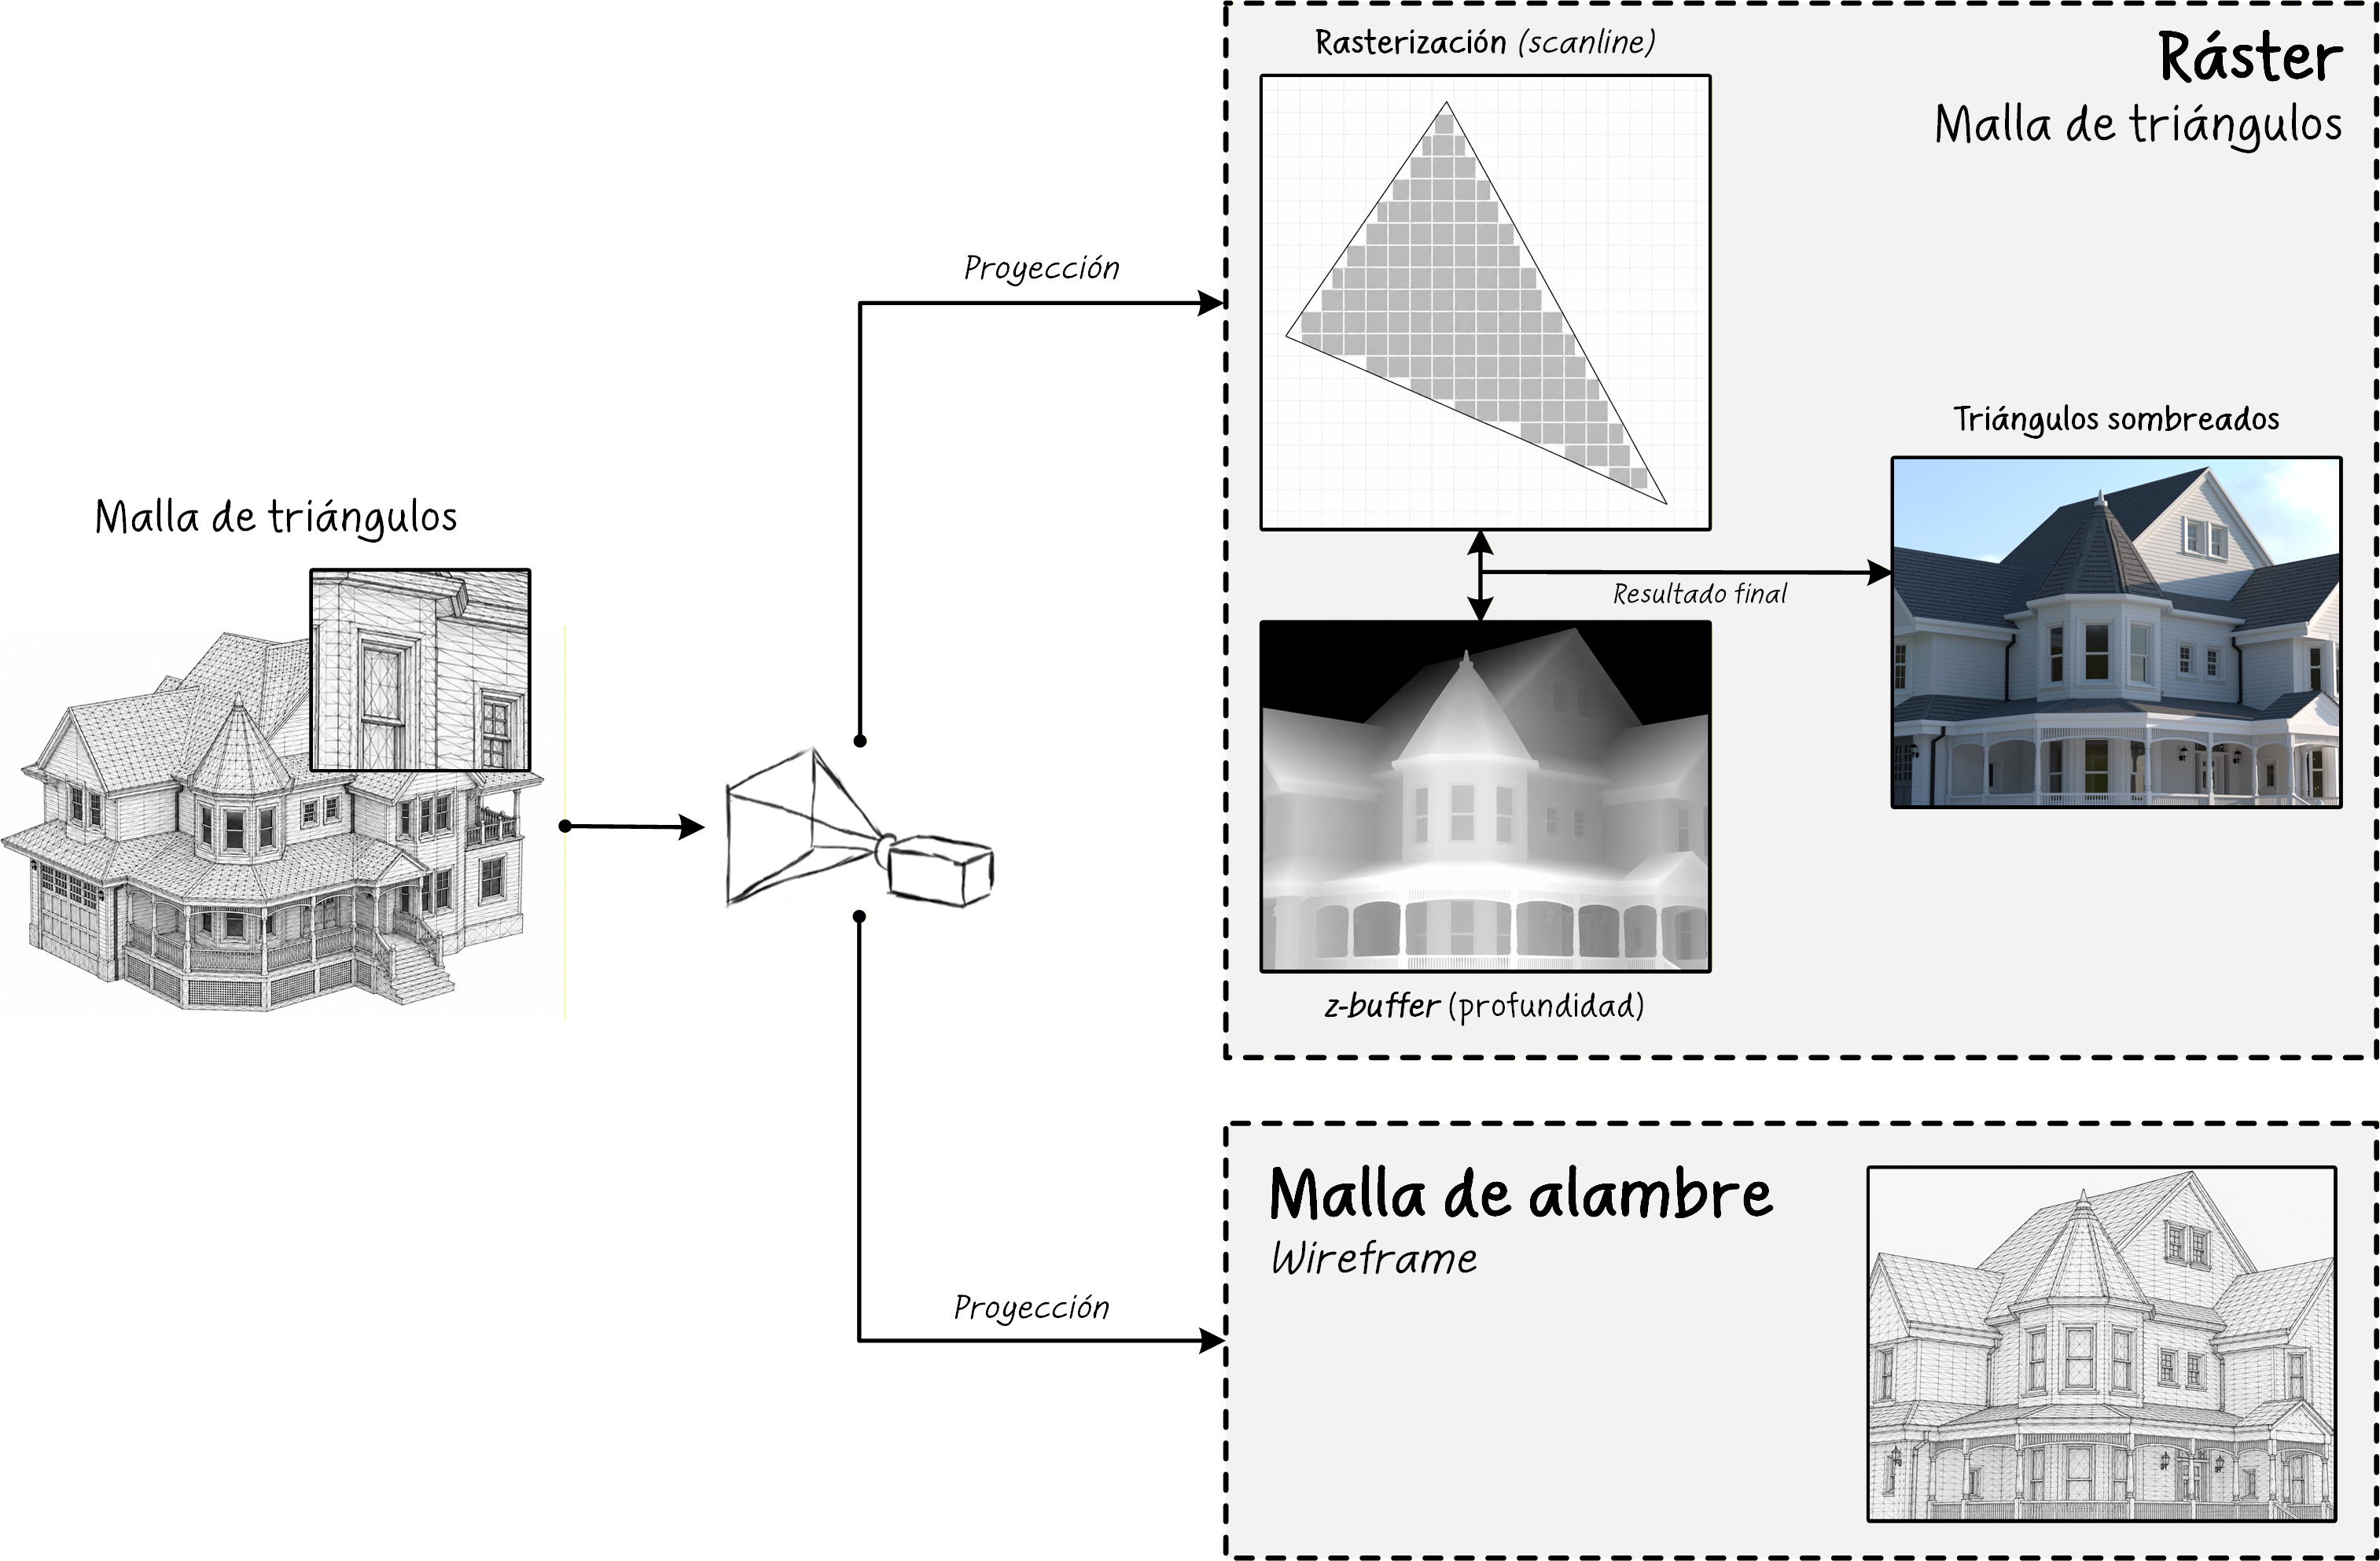
\includegraphics[width=1\linewidth,height=\textheight,keepaspectratio]{../resources/practica9/images/schema.png}

\section{El visualizador}

\label{el-visualizador}

\subsection{Importando el visualizador}

\label{importando-el-visualizador}

El visualizador de la práctica se puede descargar desde \href{../resources/practica9/visualizador.zip}{ aquí}. Copia esa carpeta a tu \emph{workspace} de Eclipse. Si quieres, puedes renombrarla como \texttt{PracticaVisualizador} para que coincida con el nombre usado en este guion.

Cuando abras un modelo \texttt{.obj} por primera vez, el visualizador puede crear junto a él un archivo \texttt{.obj.vbin}. Es una caché binaria para que las siguientes cargas sean más rápidas; si borras la caché, el visualizador la genera de nuevo.

\begin{tcolorbox}[enhanced jigsaw, colframe=quarto-callout-note-color-frame, arc=.35mm, bottomrule=.15mm, left=2mm, breakable, opacityback=0, coltitle=black, bottomtitle=1mm, toptitle=1mm, titlerule=0mm, toprule=.15mm, rightrule=.15mm, title={Descarga}, colbacktitle=quarto-callout-note-color!10!white, opacitybacktitle=0.6, colback=white, leftrule=.75mm]

El enlace de descarga también se encuentra disponible en \emph{Moodle}, en la carpeta de la práctica 9.

\end{tcolorbox}

Para importar el proyecto:

\begin{enumerate}
\def\labelenumi{\arabic{enumi}.}
\tightlist
\item
  Ve a \textbf{File → Import}.
\item
  Selecciona \textbf{General → Existing projects into workspace} (ver Figura~\ref{fig-import}).
\item
  Elige la carpeta \texttt{visualizador} (o \texttt{PracticaVisualizador}, si la has renombrado).
\end{enumerate}

\begin{figure}

\centering{

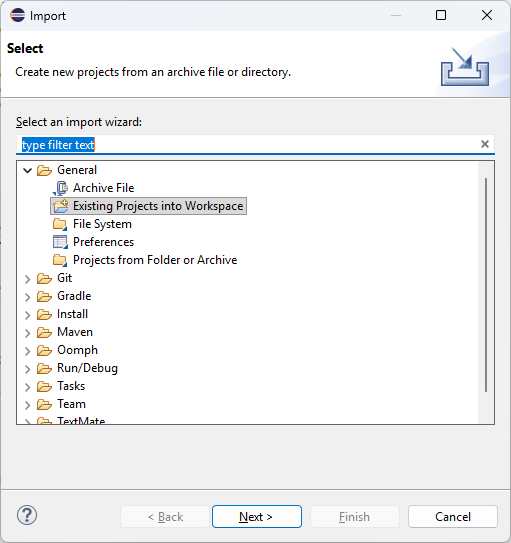
\includegraphics[width=0.6\linewidth,height=\textheight,keepaspectratio]{../resources/practica9/images/import_eclipse.png}

}

\caption{\label{fig-import}Ventana para importar proyecto.}

\end{figure}%

\subsection{El código fuente: organización por paquetes}

\label{el-código-fuente-organización-por-paquetes}

El visualizador es una aplicación suficientemente grande como para que resulte necesario agrupar las clases en \textbf{paquetes}. Un paquete es un conjunto de clases que representan conceptos relacionados entre sí.

El código fuente está dividido en cinco paquetes:

\begin{itemize}
\tightlist
\item
  \textbf{\texttt{app}}: arranque del programa y archivo \texttt{Configuracion}, pensado para cambios sencillos.
\item
  \textbf{\texttt{geometria}}: clases que representan elementos geométricos como puntos, vectores, normales, caras, objetos y matrices de transformación.
\item
  \textbf{\texttt{escena}}: clases que representan los elementos de la escena, como colores, materiales, luces y la cámara.
\item
  \textbf{\texttt{interfaz}}: clases que representan el interfaz gráfico, incluyendo la ventana principal y los paneles de visualización y configuración.
\item
  \textbf{\texttt{renderer}}: rasterizado, sombreado y efectos visuales. No hace falta entrar aquí al principio.
\end{itemize}

Puedes ver estos paquetes en el explorador de paquetes de Eclipse, en la parte izquierda de la pantalla (Figura~\ref{fig-packages}). En el sistema de archivos, cada paquete se corresponde con una carpeta dentro de la carpeta del proyecto.

\begin{figure}

\centering{

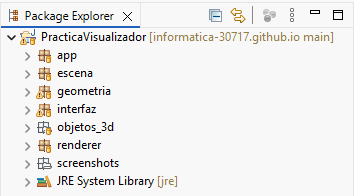
\includegraphics[width=0.4\linewidth,height=\textheight,keepaspectratio]{../resources/practica9/images/package_view.png}

}

\caption{\label{fig-packages}Paquetes del proyecto en Eclipse.}

\end{figure}%

También puedes crear un paquete nuevo para organizar tu código, pero ten cuidado con los cambios que eso puede suponer en el resto del proyecto. En Java, cada clase tiene un nombre completo que incluye el paquete al que pertenece. Por ejemplo, la clase \texttt{Luz} del paquete \texttt{escena} se llama \texttt{escena.Luz}. Si la mueves a otro paquete, su nombre completo cambiará y habrá que actualizar todas las referencias a esa clase en el código.

Para crear un nuevo proyecto puedes hacer click derecho sobre el proyecto en el explorador de paquetes, seleccionar \textbf{New → Package}, darle un nombre y pulsar \textbf{Finish} (Figura~\ref{fig-new-package}).

\begin{figure}

\centering{

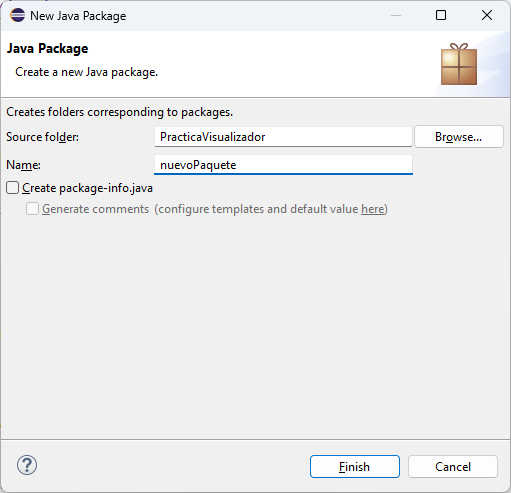
\includegraphics[width=0.6\linewidth,height=\textheight,keepaspectratio]{../resources/practica9/images/new_package.png}

}

\caption{\label{fig-new-package}Creación de un nuevo paquete en Eclipse.}

\end{figure}%

Para mover una clase a otro paquete, arrástrala y suéltala en el nuevo paquete. Antes de confirmar, asegúrate de que está marcada la opción \textbf{\emph{Update references to \texttt{\textless{}clase\textgreater{}.java}}} para que \emph{Eclipse} actualice automáticamente todas las referencias a esa clase en el código. Antes de confirmar, puedes pulsar \textbf{Preview} para ver qué cambios se realizarían en todo el código del proyecto, como se muestra en la Figura~\ref{fig-preview-move}.

\begin{figure}

\centering{

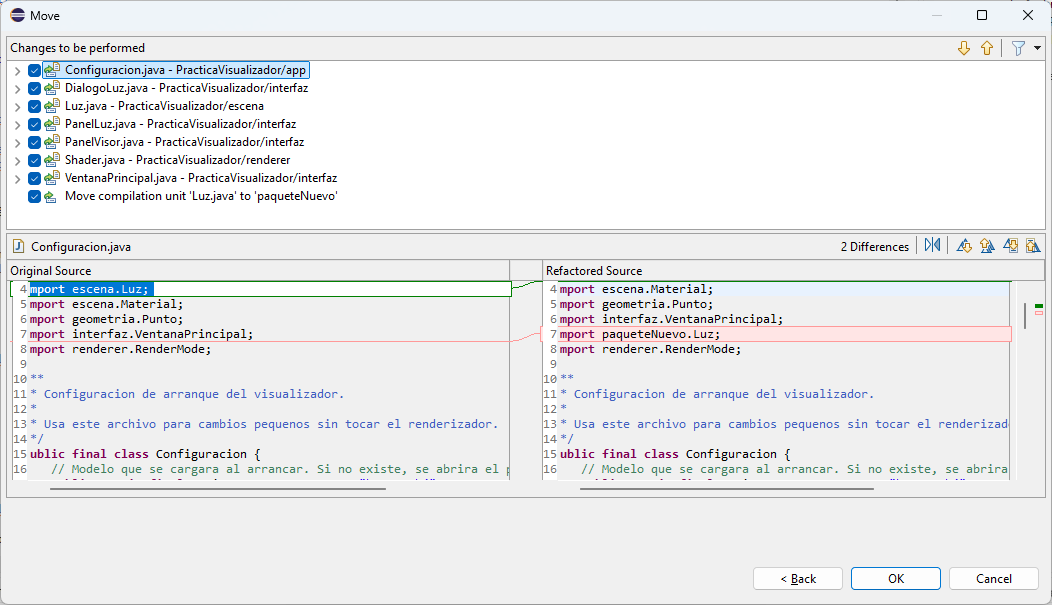
\includegraphics[width=1\linewidth,height=\textheight,keepaspectratio]{../resources/practica9/images/preview_changes.png}

}

\caption{\label{fig-preview-move}Vista previa de los cambios al mover una clase a otro paquete.}

\end{figure}%

\begin{tcolorbox}[enhanced jigsaw, colframe=quarto-callout-note-color-frame, arc=.35mm, bottomrule=.15mm, left=2mm, breakable, opacityback=0, coltitle=black, bottomtitle=1mm, toptitle=1mm, titlerule=0mm, toprule=.15mm, rightrule=.15mm, title={Experimenta con los paquetes}, colbacktitle=quarto-callout-note-color!10!white, opacitybacktitle=0.6, colback=white, leftrule=.75mm]

Crea un paquete nuevo: haz clic derecho sobre el proyecto y ve a \textbf{New → Package}. Ponle el nombre que quieras y pulsa \textbf{Finish}.

Después, arrastra y suelta \texttt{Luz.java} del paquete \texttt{escena} al nuevo paquete. Antes de confirmar, asegúrate de que está marcada la opción \textbf{\emph{Update references to \texttt{Luz.java}}} y pulsa \textbf{Preview} para ver qué cambios se realizarían en todo el código del proyecto. Una vez revisados, vuelve a dejar \texttt{Luz.java} en \texttt{escena} y borra el paquete que has creado (botón derecho → \textbf{Delete}).

\textbf{¿Por qué esos cambios de código?} Cuando desde un archivo quieres acceder a una clase de otro paquete, tienes dos opciones: o escribir \texttt{\textless{}paquete\textgreater{}.\textless{}clase\textgreater{}}, o bien poner al principio \texttt{import\ \textless{}paquete\textgreater{}.\textless{}clase\textgreater{}} y usar simplemente \texttt{\textless{}clase\textgreater{}}.

\end{tcolorbox}

\subsection{El código fuente: programación orientada a objetos}

\label{el-código-fuente-programación-orientada-a-objetos}

La regla habitual de la programación orientada a objetos es que cada archivo contiene una clase, y cada clase representa un concepto concreto.

En el paquete \texttt{geometria} hay tres clases geométricas básicas:

\begin{itemize}
\tightlist
\item
  \textbf{\texttt{Punto}}: punto en el espacio (vector de 3 componentes).
\item
  \textbf{\texttt{Direccion}}: dirección en el espacio (vector de 3 componentes).
\item
  \textbf{\texttt{Normal}}: normal en el espacio, dirección de longitud 1.
\end{itemize}

Un \textbf{\texttt{Objeto}} es una serie de caras y vértices. Un vértice es un punto junto con su normal, y una \textbf{\texttt{Cara}} es una lista de vértices con aristas entre puntos consecutivos (y entre el último y el primero).

\begin{tcolorbox}[enhanced jigsaw, colframe=quarto-callout-note-color-frame, arc=.35mm, bottomrule=.15mm, left=2mm, breakable, opacityback=0, coltitle=black, bottomtitle=1mm, toptitle=1mm, titlerule=0mm, toprule=.15mm, rightrule=.15mm, title={Explora el código}, colbacktitle=quarto-callout-note-color!10!white, opacitybacktitle=0.6, colback=white, leftrule=.75mm]

\begin{itemize}
\tightlist
\item
  Abre en Eclipse los archivos de las clases \texttt{Punto}, \texttt{Direccion} y \texttt{Normal}. Repasa el código de cada una y observa cómo se relaciona con el \emph{Outline} que aparece a la derecha, que muestra esquemáticamente los atributos y métodos de la clase.
\end{itemize}

\begin{figure}[H]

\centering{

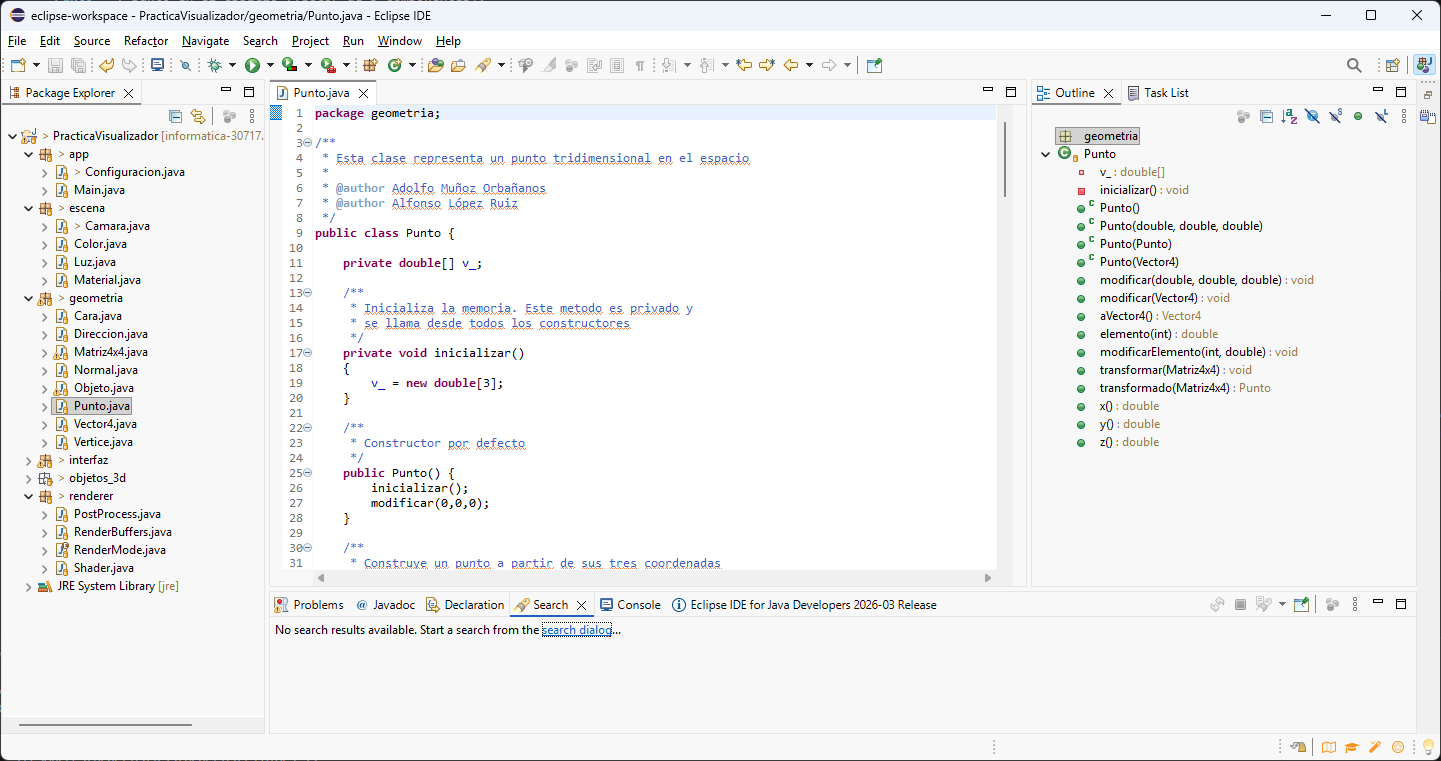
\includegraphics[width=1\linewidth,height=\textheight,keepaspectratio]{../resources/practica9/images/punto_outline.png}

}

\caption{\label{fig-outline}\emph{Outline} de \emph{Eclipse} (derecha) mostrando los métodos de la clase \texttt{Punto}.}

\end{figure}%

\begin{itemize}
\tightlist
\item
  \textbf{¿En qué clase está el método \texttt{public\ static\ void\ main(String{[}{]}\ args)}?} Sólo puede haber uno por aplicación; búscalo (pista: está en el paquete \texttt{app}).
\end{itemize}

\end{tcolorbox}

\subsection{Ejecutando el visualizador}

\label{ejecutando-el-visualizador}

Ejecuta el visualizador desde Eclipse usando \texttt{app.Main} (\textbf{Run As → Java Application}). Al arrancar, el programa cargará el modelo configurado en \texttt{app.Configuracion}. Para cargar otro objeto tridimensional, ve a \textbf{Archivo → Abrir modelo} y selecciona un archivo \texttt{.obj} de la carpeta \texttt{objetos\_3d} del proyecto. Te recomendamos empezar con \texttt{house.obj} o \texttt{trex.obj}. La carga puede tardar unos segundos.

Puedes cambiar el modo de visualización entre \textbf{Malla de alambre} (\emph{wireframe}), donde sólo se muestran las aristas, y \textbf{\emph{Raster}}, que rellena las caras con iluminación.

\begin{tcolorbox}[enhanced jigsaw, colframe=quarto-callout-note-color-frame, arc=.35mm, bottomrule=.15mm, left=2mm, breakable, opacityback=0, coltitle=black, bottomtitle=1mm, toptitle=1mm, titlerule=0mm, toprule=.15mm, rightrule=.15mm, title={Experimenta con el visualizador}, colbacktitle=quarto-callout-note-color!10!white, opacitybacktitle=0.6, colback=white, leftrule=.75mm]

\begin{itemize}
\tightlist
\item
  Prueba a cambiar los diferentes parámetros de la cámara o a activar el \emph{backface culling}. ¿Qué ocurre?
\item
  En modo \textbf{\emph{Raster}}, cambia las propiedades del material (\textbf{Escena → Material}). Intenta conseguir que el objeto sea de color amarillo.
\item
  Juega también con las propiedades de la luz (\textbf{Escena → Luz}).
\end{itemize}

\end{tcolorbox}

\subsection{Primeros cambios de código}

\label{primeros-cambios-de-código}

Si vas a tocar código por primera vez, empieza por \texttt{app.Configuracion}. Ese archivo concentra los cambios sencillos del proyecto: modelo inicial, modo de visualización, orientación inicial de la cámara, material y luz.

\begin{tcolorbox}[enhanced jigsaw, colframe=quarto-callout-note-color-frame, arc=.35mm, bottomrule=.15mm, left=2mm, breakable, opacityback=0, coltitle=black, bottomtitle=1mm, toptitle=1mm, titlerule=0mm, toprule=.15mm, rightrule=.15mm, title={Personaliza el arranque}, colbacktitle=quarto-callout-note-color!10!white, opacitybacktitle=0.6, colback=white, leftrule=.75mm]

Abre \texttt{app.Configuracion} y prueba cambios pequeños, sin salirte de ese archivo:

\begin{itemize}
\tightlist
\item
  cambia \texttt{MODELO\_INICIAL} por otro \texttt{.obj};
\item
  prueba otro \texttt{MODO\_INICIAL};
\item
  modifica el color del material o de la luz;
\item
  cambia el campo de visión, la inclinación o la rotación inicial de la cámara.
\end{itemize}

Ten en cuenta que el visualizador calcula automáticamente una distancia base al cargar o recentrar un modelo, pero no compensa el campo de visión configurado. Así, al cambiar \texttt{CAMARA\_FOV} deberías notar de verdad cómo se abre o se cierra la vista.

Ejecuta de nuevo el programa.

\end{tcolorbox}

\subsection{Depuración de errores}

\label{depuración-de-errores}

En aplicaciones de este tamaño, el depurador de \emph{Eclipse} resulta muy útil para entender paso a paso qué hace el código. Vamos a depurar el método \texttt{matrizDeProyeccion()} de la clase \texttt{PanelVisor} del paquete \texttt{interfaz}.

No hace falta leer toda la clase antes: usa el buscador de \emph{Eclipse} y salta directamente a ese método.

\begin{tcolorbox}[enhanced jigsaw, colframe=quarto-callout-note-color-frame, arc=.35mm, bottomrule=.15mm, left=2mm, breakable, opacityback=0, coltitle=black, bottomtitle=1mm, toptitle=1mm, titlerule=0mm, toprule=.15mm, rightrule=.15mm, title={Usa el depurador}, colbacktitle=quarto-callout-note-color!10!white, opacitybacktitle=0.6, colback=white, leftrule=.75mm]

\begin{enumerate}
\def\labelenumi{\arabic{enumi}.}
\item
  Busca en \texttt{PanelVisor} la línea:

  \PracticeCode{../resources/practica9/snippets/projection-matrix-breakpoint.java}
\item
  Pon un \textbf{punto de ruptura} (\emph{breakpoint}): botón derecho sobre la línea → \textbf{\emph{Toggle Breakpoint}}.
\item
  Ejecuta la aplicación en \textbf{modo depuración}.
\item
  Pulsa \textbf{\texttt{F6}} unas pocas veces para avanzar paso a paso y observa cómo se va construyendo la matriz de proyección.
\item
  Pulsa \textbf{\texttt{F8}} para continuar la ejecución normal del programa.
\item
  ¿Por qué el programa vuelve una y otra vez a esa misma línea aunque no hayas hecho nada?
\item
  Cuando termines, desactiva el \emph{breakpoint}: botón derecho → \textbf{Disable Breakpoint}.
\end{enumerate}

\end{tcolorbox}

\section{El visualizador por dentro}

\label{el-visualizador-por-dentro}

\begin{tcolorbox}[enhanced jigsaw, colframe=quarto-callout-note-color-frame, arc=.35mm, bottomrule=.15mm, left=2mm, breakable, opacityback=0, coltitle=black, bottomtitle=1mm, toptitle=1mm, titlerule=0mm, toprule=.15mm, rightrule=.15mm, title={Idea clave}, colbacktitle=quarto-callout-note-color!10!white, opacitybacktitle=0.6, colback=white, leftrule=.75mm]

En esta parte no hace falta memorizar matrices ni seguir todas las fórmulas al detalle. Quédate con esta idea: el programa coloca el objeto respecto a la cámara, proyecta los puntos sobre la pantalla, decide qué partes se ven y les asigna un color.

Con esa intuición ya puedes entender lo esencial del visualizador y trabajar con el proyecto sin perderte en la matemática.

\end{tcolorbox}

\subsection{Proyectando 3 dimensiones en 2 dimensiones}

\label{proyectando-3-dimensiones-en-2-dimensiones}

Piensa en este paso como una traducción: del modelo 3D a la imagen 2D que termina apareciendo en pantalla. El programa toma cada punto del objeto, lo sitúa respecto a la cámara y calcula dónde debe dibujarse.

En el código esa traducción se implementa con \textbf{matrices de cuatro dimensiones} (clase \texttt{Matriz4x4}). No hace falta memorizar la técnica: basta con saber que permite encadenar traslaciones, giros y perspectiva de una forma uniforme. Para ello, a cada punto se le añade una cuarta componente llamada \textbf{coordenada homogénea}:

\[
(x,\, y,\, z) \;\longrightarrow\; (x,\, y,\, z,\, 1)
\]

La clase \texttt{Vector4} representa ese vector de 4 dimensiones. La transformación de un vector respecto a una matriz es un producto:

\[
V_t = M \cdot V
\]

donde \(V_t\) es el vector transformado, \(M\) la matriz y \(V\) el vector original. Para recuperar el punto 3D se divide por la coordenada homogénea \(w\):

\[
(x,\, y,\, z,\, w) \;\longrightarrow\; \left(\frac{x}{w},\;\frac{y}{w},\;\frac{z}{w}\right)
\]

Si \(w = 0\), ese \texttt{Vector4} no representa un punto que puedas recuperar con la división anterior, sino una \textbf{dirección}. Por eso una traslación no le afecta. Por ejemplo:

\[
\begin{pmatrix}
1 & 0 & 0 & 10\\
0 & 1 & 0 & 0\\
0 & 0 & 1 & 0\\
0 & 0 & 0 & 1
\end{pmatrix}
\cdot
\begin{pmatrix}4\\3\\2\\1\end{pmatrix}
=
\begin{pmatrix}14\\3\\2\\1\end{pmatrix}
\qquad
\begin{pmatrix}
1 & 0 & 0 & 10\\
0 & 1 & 0 & 0\\
0 & 0 & 1 & 0\\
0 & 0 & 0 & 1
\end{pmatrix}
\cdot
\begin{pmatrix}4\\3\\2\\0\end{pmatrix}
=
\begin{pmatrix}4\\3\\2\\0\end{pmatrix}
\]

En el primer caso se ha movido el punto diez unidades en \(x\). En el segundo, la misma operación no cambia el vector: con \(w = 0\) la parte de traslación queda multiplicada por cero. Si lo que querías era mover una posición, entonces ese vector debía tener \(w = 1\).

\begin{tcolorbox}[enhanced jigsaw, colframe=quarto-callout-note-color-frame, arc=.35mm, bottomrule=.15mm, left=2mm, breakable, opacityback=0, coltitle=black, bottomtitle=1mm, toptitle=1mm, titlerule=0mm, toprule=.15mm, rightrule=.15mm, title={Busca en el código}, colbacktitle=quarto-callout-note-color!10!white, opacitybacktitle=0.6, colback=white, leftrule=.75mm]

¿Qué dos métodos de la clase \texttt{Punto} encapsulan respectivamente la conversión \((x,y,z) \to (x,y,z,1)\) y la vuelta \((x,y,z,w) \to (x/w,\,y/w,\,z/w)\)? Estudia su código.

\end{tcolorbox}

\subsection{Matrices de transformación}

\label{matrices-de-transformación}

Las operaciones importantes aquí son muy intuitivas: trasladar un objeto, cambiar su tamaño y girarlo. La clase \texttt{Matriz4x4} tiene un método para cada una. No hace falta memorizar las matrices; úsalas como una forma compacta de expresar esas transformaciones:

\[
\text{traslacion}(x,y,z) \;\to\; \begin{pmatrix} 1 & 0 & 0 & x \\ 0 & 1 & 0 & y \\ 0 & 0 & 1 & z \\ 0 & 0 & 0 & 1 \end{pmatrix}
\qquad
\text{escalado}(x,y,z) \;\to\; \begin{pmatrix} x & 0 & 0 & 0 \\ 0 & y & 0 & 0 \\ 0 & 0 & z & 0 \\ 0 & 0 & 0 & 1 \end{pmatrix}
\]

\[
\text{rotacionX}(a) \;\to\; \begin{pmatrix} 1 & 0 & 0 & 0 \\ 0 & \cos a & \sin a & 0 \\ 0 & {-\sin a} & \cos a & 0 \\ 0 & 0 & 0 & 1 \end{pmatrix}
\qquad
\text{rotacionY}(a) \;\to\; \begin{pmatrix} \cos a & 0 & {-\sin a} & 0 \\ 0 & 1 & 0 & 0 \\ \sin a & 0 & \cos a & 0 \\ 0 & 0 & 0 & 1 \end{pmatrix}
\]

\[
\text{rotacionZ}(a) \;\to\; \begin{pmatrix} \cos a & \sin a & 0 & 0 \\ {-\sin a} & \cos a & 0 & 0 \\ 0 & 0 & 1 & 0 \\ 0 & 0 & 0 & 1 \end{pmatrix}
\]

La versión HTML incluye una visualización interactiva de \texttt{rotacionZ}. En PDF, quédate con este caso fijo para \(a=35^\circ\):

\begin{longtable}[]{@{}lr@{}}
\toprule\noalign{}
Magnitud & Valor aproximado \\
\midrule\noalign{}
\endhead
\bottomrule\noalign{}
\endlastfoot
\(\cos a\) & 0.819 \\
\(\sin a\) & 0.574 \\
Punto inicial & \((0.72,\ 0.24,\ 0.38)\) \\
Punto rotado & \((0.45,\ 0.61,\ 0.38)\) \\
\end{longtable}

La rotación respecto al eje Z cambia las coordenadas \(x\) e \(y\), pero mantiene constante la coordenada \(z\).

\subsection{La proyección en perspectiva}

\label{la-proyección-en-perspectiva}

Aquí aparece un efecto que ya conoces de la fotografía: \textbf{los objetos lejanos se ven más pequeños, y cambiar la focal cambia cuánto abarca la cámara}.

En el visor sucede lo mismo. Primero se coloca el objeto con respecto a la cámara, después se aplica la perspectiva y al final se convierten las coordenadas a píxeles de la pantalla. Si solo quieres quedarte con una idea, quédate con que \textbf{una distancia focal mayor cierra la vista, mientras que una distancia focal menor la abre}.

\begin{figure}

\begin{minipage}{0.33\linewidth}

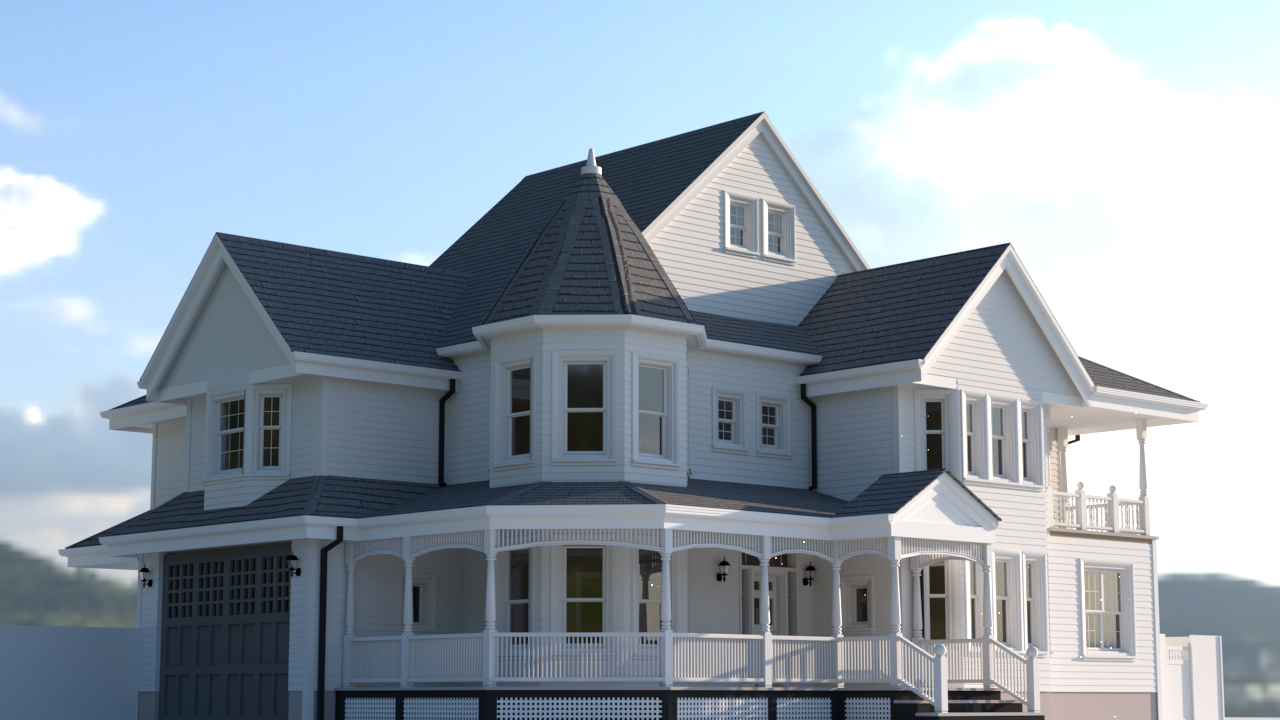
\includegraphics[width=1\linewidth,height=\textheight,keepaspectratio]{../resources/practica9/images/house_65mm.png}

\subcaption{\label{}65 mm: encuadre amplio.}
\end{minipage}%
%
\begin{minipage}{0.33\linewidth}

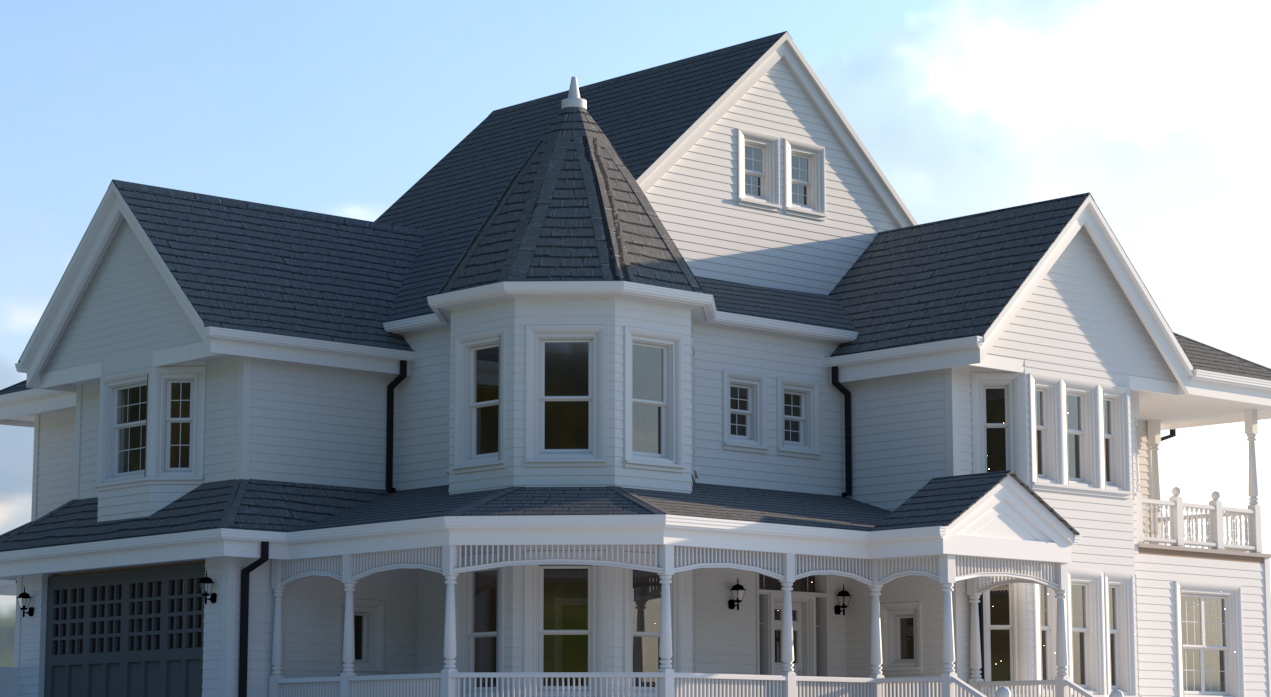
\includegraphics[width=1\linewidth,height=\textheight,keepaspectratio]{../resources/practica9/images/house_80mm.png}

\subcaption{\label{}80 mm: vista de referencia.}
\end{minipage}%
%
\begin{minipage}{0.33\linewidth}

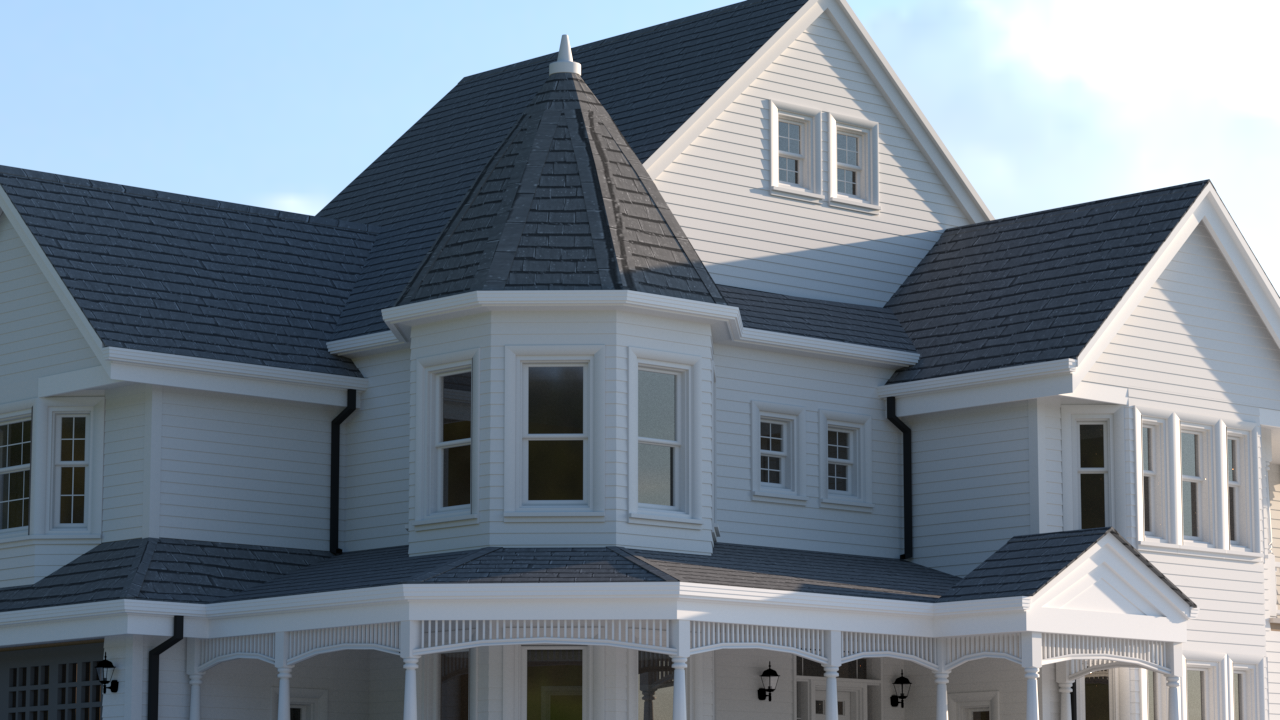
\includegraphics[width=1\linewidth,height=\textheight,keepaspectratio]{../resources/practica9/images/house_100mm.png}

\subcaption{\label{}100 mm: encuadre estrecho.}
\end{minipage}%

\caption{\label{fig-practica9-focal}A mayor distancia focal, menor campo de visión y mayor imagen proyectada sobre el sensor.}

\end{figure}%

Una manera muy simple de resumirlo es esta:

\[
x' = \frac{f\,x}{z}; y' = \frac{f\,y}{z}
\]

Cuanto mayor es \(z\) (más lejos está el punto), menor aparece en pantalla. El resto de fórmulas del programa refinan esa misma idea para trabajar con una cámara completa, su campo de visión y el tamaño de la ventana.

\begin{tcolorbox}[enhanced jigsaw, colframe=quarto-callout-tip-color-frame, arc=.35mm, bottomrule=.15mm, left=2mm, breakable, opacityback=0, coltitle=black, bottomtitle=1mm, toptitle=1mm, titlerule=0mm, toprule=.15mm, rightrule=.15mm, title={Detalle técnico opcional}, colbacktitle=quarto-callout-tip-color!10!white, opacitybacktitle=0.6, colback=white, leftrule=.75mm]

La \textbf{matriz de perspectiva} transforma coordenadas de cámara a coordenadas de recorte (\emph{clip space}):

\[
\text{perspectiva}(fov,ar,n,f) \;\to\; \begin{pmatrix} (ar\cdot\tan(fov/2))^{-1} & 0 & 0 & 0 \\ 0 & \tan(fov/2)^{-1} & 0 & 0 \\ 0 & 0 & \frac{f}{f-n} & -\frac{nf}{f-n} \\ 0 & 0 & 1 & 0 \end{pmatrix}
\]

con \(n = 1\), \(f = 100\), \(ar = h/w\) y \(fov\) el ángulo de campo de visión. La \textbf{matriz de pantalla} convierte coordenadas normalizadas a píxeles:

\[
\text{pantalla}(w,h) \;\to\; \begin{pmatrix} w/2 & 0 & 0 & w/2 \\ 0 & h/2 & 0 & h/2 \\ 0 & 0 & 1 & 0 \\ 0 & 0 & 0 & 1 \end{pmatrix}
\]

La \textbf{matriz de proyección completa} que aplica \texttt{PanelVisor} a todos los puntos del objeto es:

\[
\begin{aligned}
M_p &= \text{pantalla}(w,h)\cdot\text{perspectiva}(fov,h/w,1,100) \\
    &\quad\cdot\text{traslacion}(0,0,d)\cdot\text{rotacionX}(inc) \\
    &\quad\cdot\text{rotacionY}(rot)\cdot\text{traslacion}(x_c,y_c,z_c)
\end{aligned}
\]

donde:

\begin{itemize}
\tightlist
\item
  \(d\) controla la \textbf{separación en profundidad entre la cámara y el objeto}. Si piensas en una cámara mirando al objeto que tiene delante, \(d\) indica si ese objeto queda más cerca o más lejos de la cámara.
\item
  \(inc\) es la \textbf{inclinación vertical} de la cámara: equivale a inclinar la vista hacia arriba o hacia abajo.
\item
  \(rot\) es la \textbf{rotación horizontal} de la cámara alrededor del objeto: equivale a girar la vista hacia un lado o hacia otro.
\item
  \((x_c, y_c, z_c)\) son las coordenadas del \textbf{centro del objeto}, es decir, el punto de referencia a partir del cual el programa lo coloca y lo gira.
\end{itemize}

No hace falta preocuparse aquí por el signo exacto de cada transformación. Para seguir la práctica basta con esta idea: el visualizador coloca el objeto respecto a la cámara, ajusta la orientación de la vista y después calcula cómo se proyecta en la pantalla.

\end{tcolorbox}

La versión HTML permite ajustar el sensor y la distancia focal. En PDF, este caso fijo resume la lectura de la escena:

\begin{longtable}[]{@{}lr@{}}
\toprule\noalign{}
Parámetro & Valor \\
\midrule\noalign{}
\endhead
\bottomrule\noalign{}
\endlastfoot
Ancho del sensor, \(w\) & 36 mm \\
Alto del sensor, \(h\) & 24 mm \\
Distancia focal, \(f\) & 80 mm \\
Relación de aspecto, \(w/h\) & 1.50 \\
Campo de visión horizontal & 25.36° \\
Campo de visión vertical & 17.06° \\
\end{longtable}

Si la imagen proyectada del objeto es mayor que el sensor, la proyección existe, pero el sensor solo registra una parte y el objeto aparece recortado.

\begin{tcolorbox}[enhanced jigsaw, colframe=quarto-callout-note-color-frame, arc=.35mm, bottomrule=.15mm, left=2mm, breakable, opacityback=0, coltitle=black, bottomtitle=1mm, toptitle=1mm, titlerule=0mm, toprule=.15mm, rightrule=.15mm, title={Comprueba la rotación de la cámara}, colbacktitle=quarto-callout-note-color!10!white, opacitybacktitle=0.6, colback=white, leftrule=.75mm]

En el método \texttt{matrizDeProyeccion()} de \texttt{PanelVisor}, comenta la línea:

\PracticeCode{../resources/practica9/snippets/disable-camera-inclination.java}

(añade \texttt{//} al principio) y vuelve a ejecutar. ¿Qué ha cambiado? Prueba a comentar otras líneas del mismo método.

\end{tcolorbox}

\begin{tcolorbox}[enhanced jigsaw, colframe=quarto-callout-note-color-frame, arc=.35mm, bottomrule=.15mm, left=2mm, breakable, opacityback=0, coltitle=black, bottomtitle=1mm, toptitle=1mm, titlerule=0mm, toprule=.15mm, rightrule=.15mm, title={Compruébalo con un ejemplo}, colbacktitle=quarto-callout-note-color!10!white, opacitybacktitle=0.6, colback=white, leftrule=.75mm]

Prueba con el punto \((4,\, 3,\, 2)\) y una rotación de 90° con respecto al eje Z. Puedes multiplicar el vector fila \((4\ 3\ 2\ 1)\) por la matriz correspondiente.

Recuerda que las clases que debemos utilizar son \texttt{geometria.Vector4} y \texttt{geometria.Matriz4x4}. Para representar el punto homogéneo, puedes crear un \texttt{Vector4} con valores \texttt{(4,\ 3,\ 2,\ 1)}. Para crear la matriz de rotación, puedes usar el método \texttt{rotacionZ} de \texttt{Matriz4x4}. Para multiplicar el vector por la matriz, puedes usar el método \texttt{multiplicar} de \texttt{Matriz4x4}. Los ángulos de rotación se expresan en radianes, así que para convertir 90° a radianes puedes multiplicar el ángulo por \texttt{Math.PI\ /\ 180.0}.

Puedes hacer dos cosas para comprobar el resultado de multiplicar ese punto por la matriz de rotación:

\begin{itemize}
\tightlist
\item
  Ejecuta después el código en modo depuración para comprobar cómo se realiza esa rotación en el visualizador;
\item
  O bien, muestra por pantalla los valores del punto resultante.
\end{itemize}

Por ejemplo, utiliza este código para imprimir el resultado en la consola de \emph{Eclipse}:

\PracticeCode{../resources/practica9/snippets/print-rotated-vector.java}

\end{tcolorbox}

\subsection{Modos de visualización}

\label{modos-de-visualización}

\texttt{PanelVisor} coordina la visualización del objeto. La proyección y el recorrido de caras se encuentran en esa clase, pero el cálculo del color está en \texttt{renderer.Shader} y los efectos opcionales en \texttt{renderer.PostProcess}.

Si solo quieres modificar cámara, material, luz o modo de visualización, no hace falta entrar en ese paquete todavía.

El visualizador ofrece dos modos principales. En esta práctica nos interesa sobre todo el segundo, porque es el que utiliza la iluminación de Phong del proyecto proporcionado.

\begin{itemize}
\tightlist
\item
  \textbf{Malla de alambre} (\texttt{pintarMallaAlambre}): se recorren todas las \texttt{Caras}, se transforman sus \texttt{Puntos} y se dibujan solo las aristas.
\item
  \textbf{Raster}: se rellena cada cara visible y se calcula el color de cada píxel con el modelo de iluminación de Phong. Además, se mantiene un \textbf{\emph{z-buffer}}, es decir, un registro de profundidad para que una superficie del fondo no tape a otra que está delante.
\end{itemize}

\begin{figure}

\begin{minipage}{0.50\linewidth}

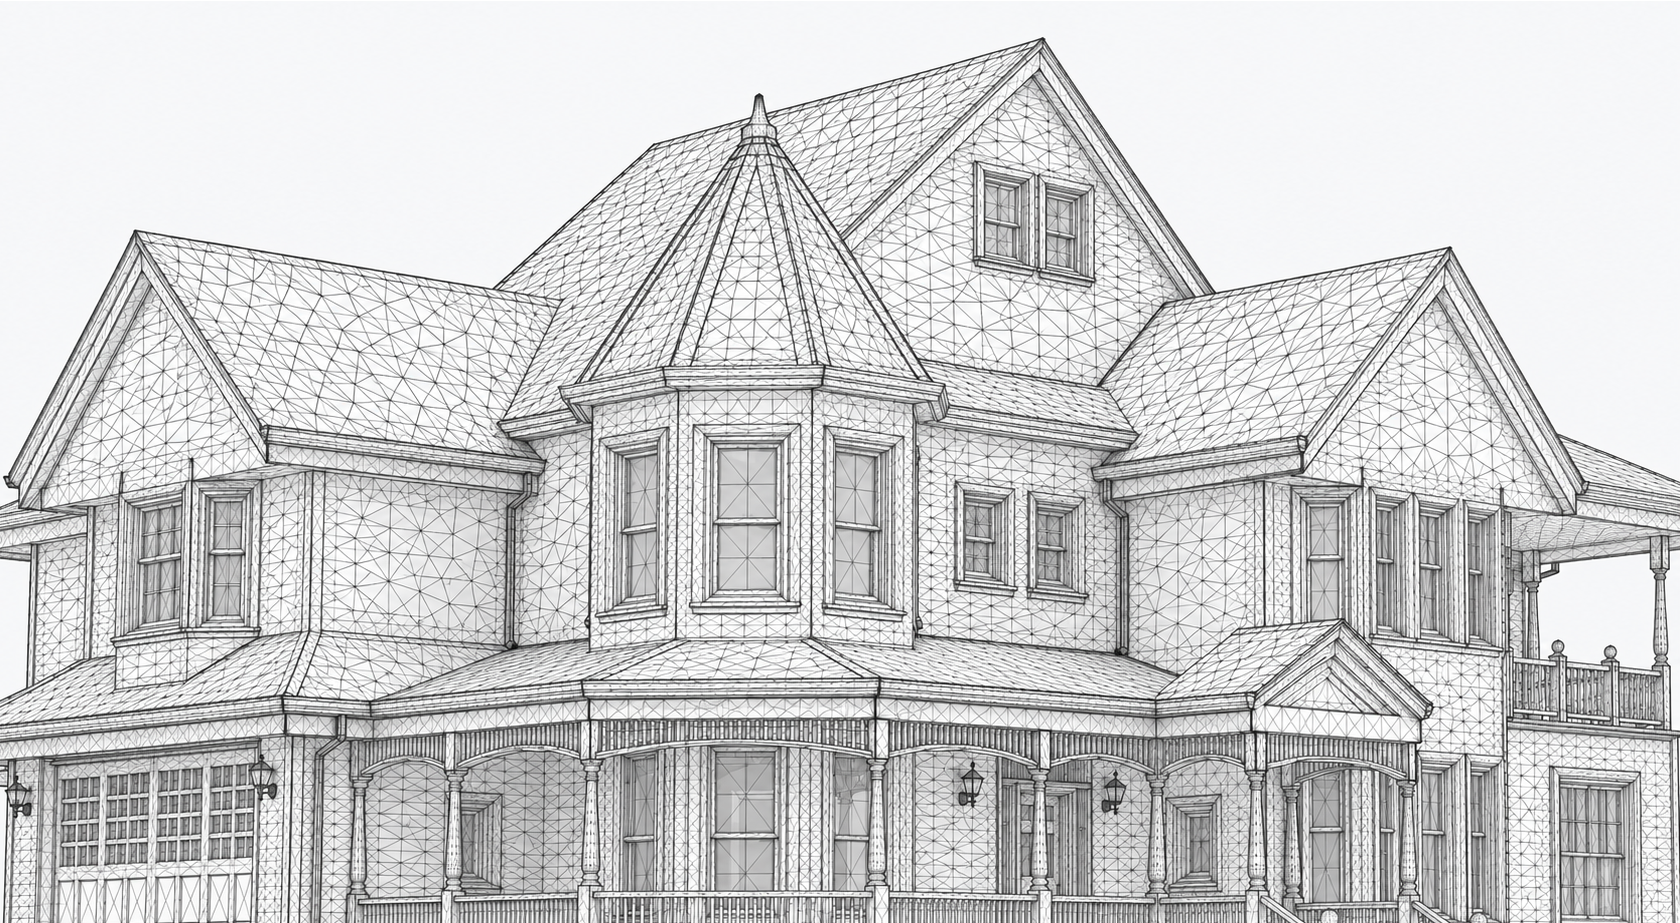
\includegraphics[width=1\linewidth,height=\textheight,keepaspectratio]{../resources/practica9/images/wireframe.png}

\subcaption{\label{}Malla de alambre.}
\end{minipage}%
%
\begin{minipage}{0.50\linewidth}

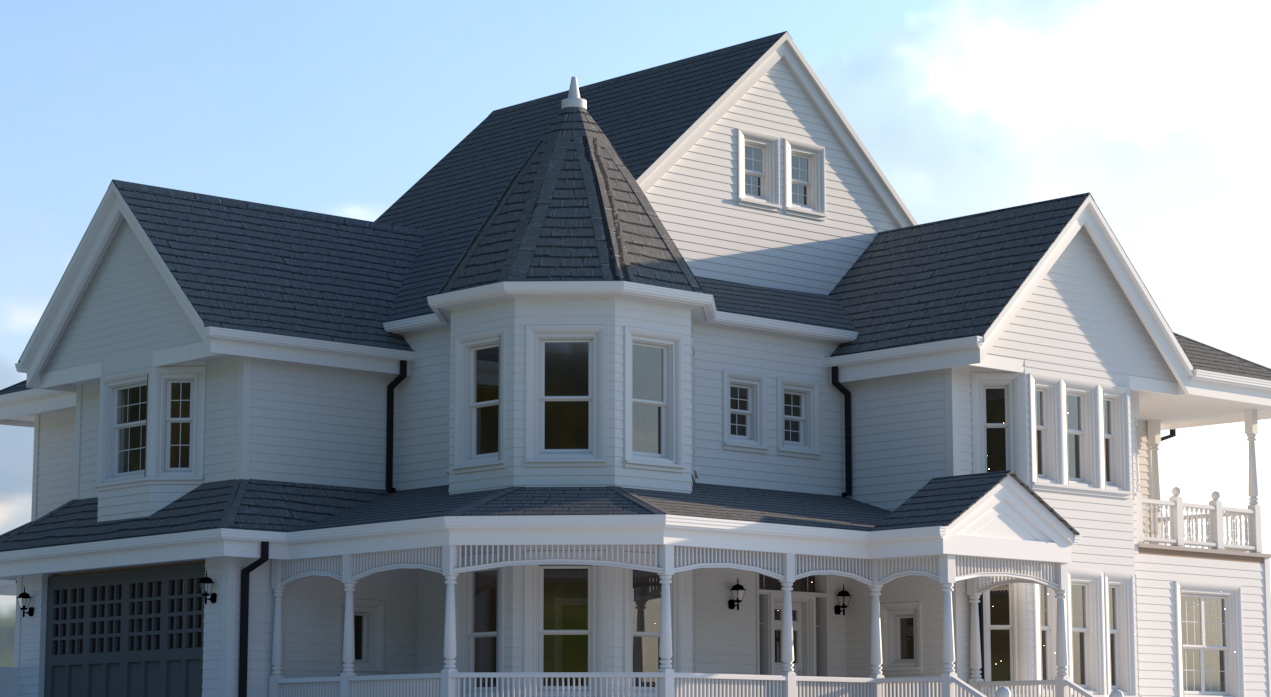
\includegraphics[width=1\linewidth,height=\textheight,keepaspectratio]{../resources/practica9/images/house_80mm.png}

\subcaption{\label{}Ráster con iluminación de Phong.}
\end{minipage}%

\caption{\label{fig-practica9-render-modes}El mismo objeto en los dos modos de visualización del programa, con focal de 80 mm.}

\end{figure}%

En ambos modos se puede activar el \textbf{\emph{backface culling}} (método \texttt{considerarCara}), que descarta las caras cuya normal apunta en sentido contrario a la cámara, acelerando el proceso de pintado.

\begin{tcolorbox}[enhanced jigsaw, colframe=quarto-callout-note-color-frame, arc=.35mm, bottomrule=.15mm, left=2mm, breakable, opacityback=0, coltitle=black, bottomtitle=1mm, toptitle=1mm, titlerule=0mm, toprule=.15mm, rightrule=.15mm, title={Busca en el código}, colbacktitle=quarto-callout-note-color!10!white, opacitybacktitle=0.6, colback=white, leftrule=.75mm]

No leas \texttt{PanelVisor} de principio a fin. Busca directamente los métodos \texttt{considerarCara}, \texttt{pintarMallaAlambre} y \texttt{pintarRaster}, y localiza después dónde se llama a \texttt{renderer.Shader} en el recorrido ráster. Identifica qué partes del algoritmo descrito en este guion implementa cada método. Compara los dos modos de visualización.

\end{tcolorbox}

\subsection{Iluminación de Phong}

\label{iluminación-de-phong}

En el modo ráster, el color de cada píxel se calcula con el \textbf{modelo de iluminación de Phong}, una aproximación clásica y muy rápida.

Puedes leerlo de forma intuitiva como la suma de tres ideas:

\begin{itemize}
\tightlist
\item
  una luz base que evita que todo quede completamente negro;
\item
  una componente difusa, que depende de cómo orientada esté la superficie hacia la luz;
\item
  una componente especular, que produce los brillos.
\end{itemize}

La iluminación de Phong se suele expresar de la siguiente manera:

\[
C_p = k_a\, C_a \;+\; k_d\, C_l\,(n_p \cdot d_l) \;+\; k_s\, C_l\,(r_p \cdot v)^{e}
\]

No hace falta memorizar todos los símbolos. En la práctica basta con relacionarlos con los controles del visualizador: \texttt{ka} añade luz base, \texttt{kd} controla la respuesta mate o difusa, \texttt{ks} refuerza el brillo y \texttt{e} hace ese brillo más abierto o más concentrado. Por otro lado, los términos \texttt{Ca} y \texttt{Cl} modelan la luz, y no el material del objeto.

La versión HTML incluye un visor 3D interactivo para cambiar \texttt{ka}, \texttt{kd}, \texttt{ks}, \texttt{e}, \texttt{Ca} y \texttt{Cl}. En PDF, la Figura~\ref{fig-practica9-phong-materials} ofrece una lectura estática de la misma idea: una superficie mate se entiende sobre todo con \texttt{kd}, mientras que una superficie brillante o metálica necesita una contribución especular mayor, controlada por \texttt{ks} y por el exponente \texttt{e}.

\begin{figure}

\begin{minipage}{0.50\linewidth}

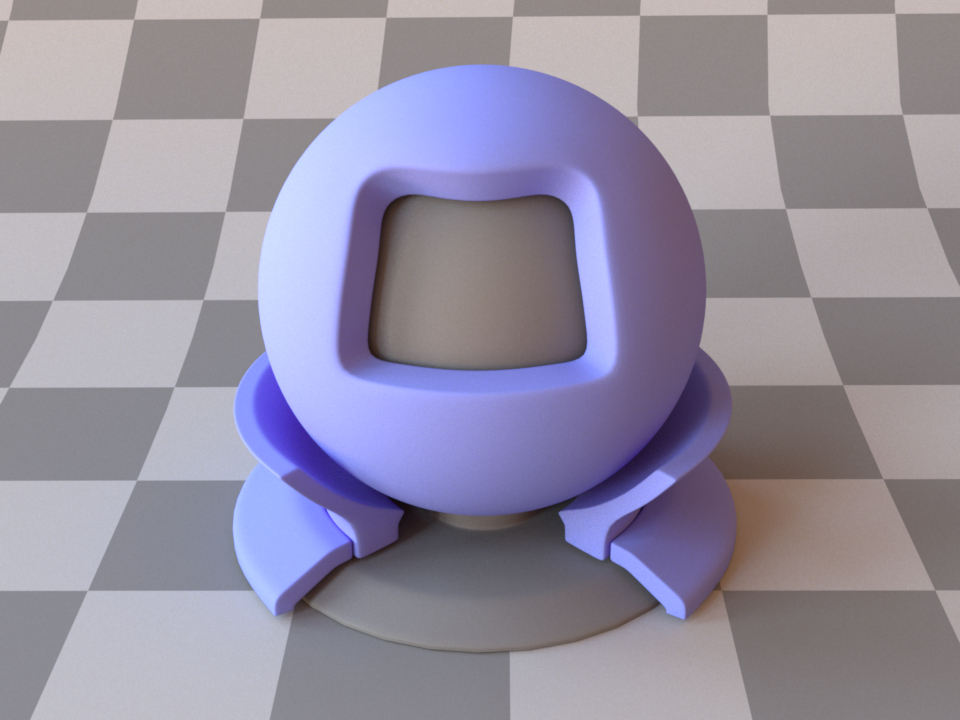
\includegraphics[width=1\linewidth,height=\textheight,keepaspectratio]{../resources/practica9/images/mitsuba_bsdf_diffuse_plain.jpg}

\subcaption{\label{}Material mate difuso.}
\end{minipage}%
%
\begin{minipage}{0.50\linewidth}

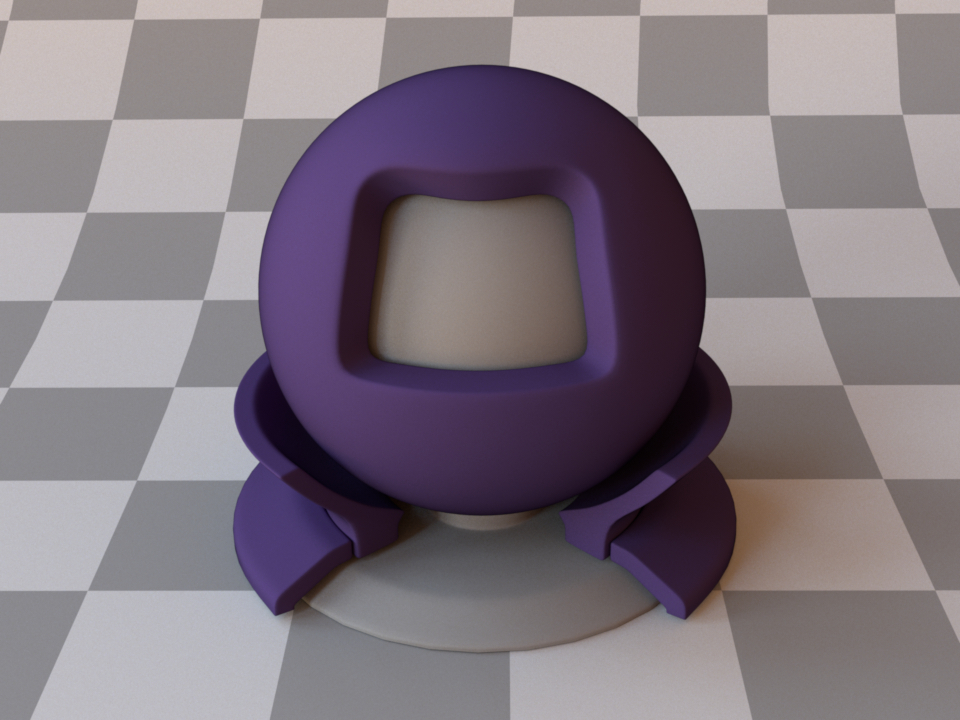
\includegraphics[width=1\linewidth,height=\textheight,keepaspectratio]{../resources/practica9/images/mitsuba_bsdf_pplastic_diffuse_component.jpg}

\subcaption{\label{}Base difusa plástica.}
\end{minipage}%
\newline
\begin{minipage}{0.50\linewidth}

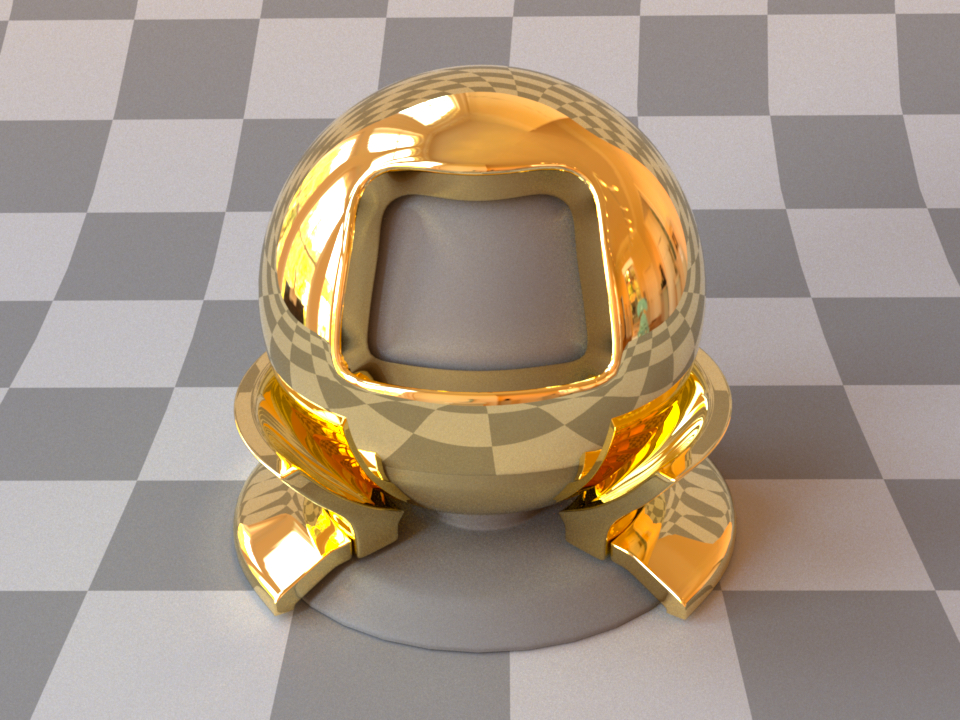
\includegraphics[width=1\linewidth,height=\textheight,keepaspectratio]{../resources/practica9/images/mitsuba_bsdf_conductor_gold.jpg}

\subcaption{\label{}Metal especular.}
\end{minipage}%
%
\begin{minipage}{0.50\linewidth}

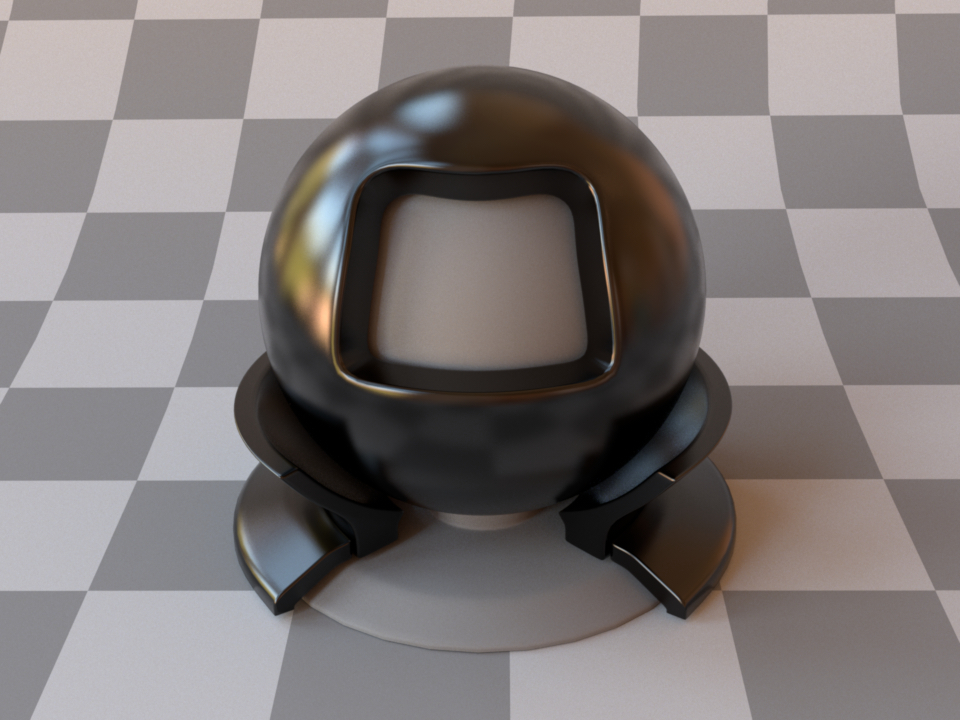
\includegraphics[width=1\linewidth,height=\textheight,keepaspectratio]{../resources/practica9/images/mitsuba_bsdf_pplastic_specular_component.jpg}

\subcaption{\label{}Brillo plástico.}
\end{minipage}%

\caption{\label{fig-practica9-phong-materials}Referencias visuales para interpretar \texttt{kd}, \texttt{ks} y \texttt{e} en el modelo de Phong. Las imágenes proceden de la documentación de Mitsuba 3 sobre materiales BSDF y se usan aquí como referencia cualitativa.}

\end{figure}%

Las siguientes imágenes no son capturas literales del visualizador, sino simplemente imágenes de apoyo para comprender mejor qué aporta cada término de la iluminación de Phong. Quédate sobre todo con estas dos ideas:

\begin{itemize}
\tightlist
\item
  Si quitas \texttt{ks}, desaparecen los brillos especulares.
\item
  Si quitas \texttt{ka}, las zonas en sombra se oscurecen mucho más.
\end{itemize}

En PDF, compara las imágenes lado a lado:

\begin{figure}

\begin{minipage}{0.50\linewidth}

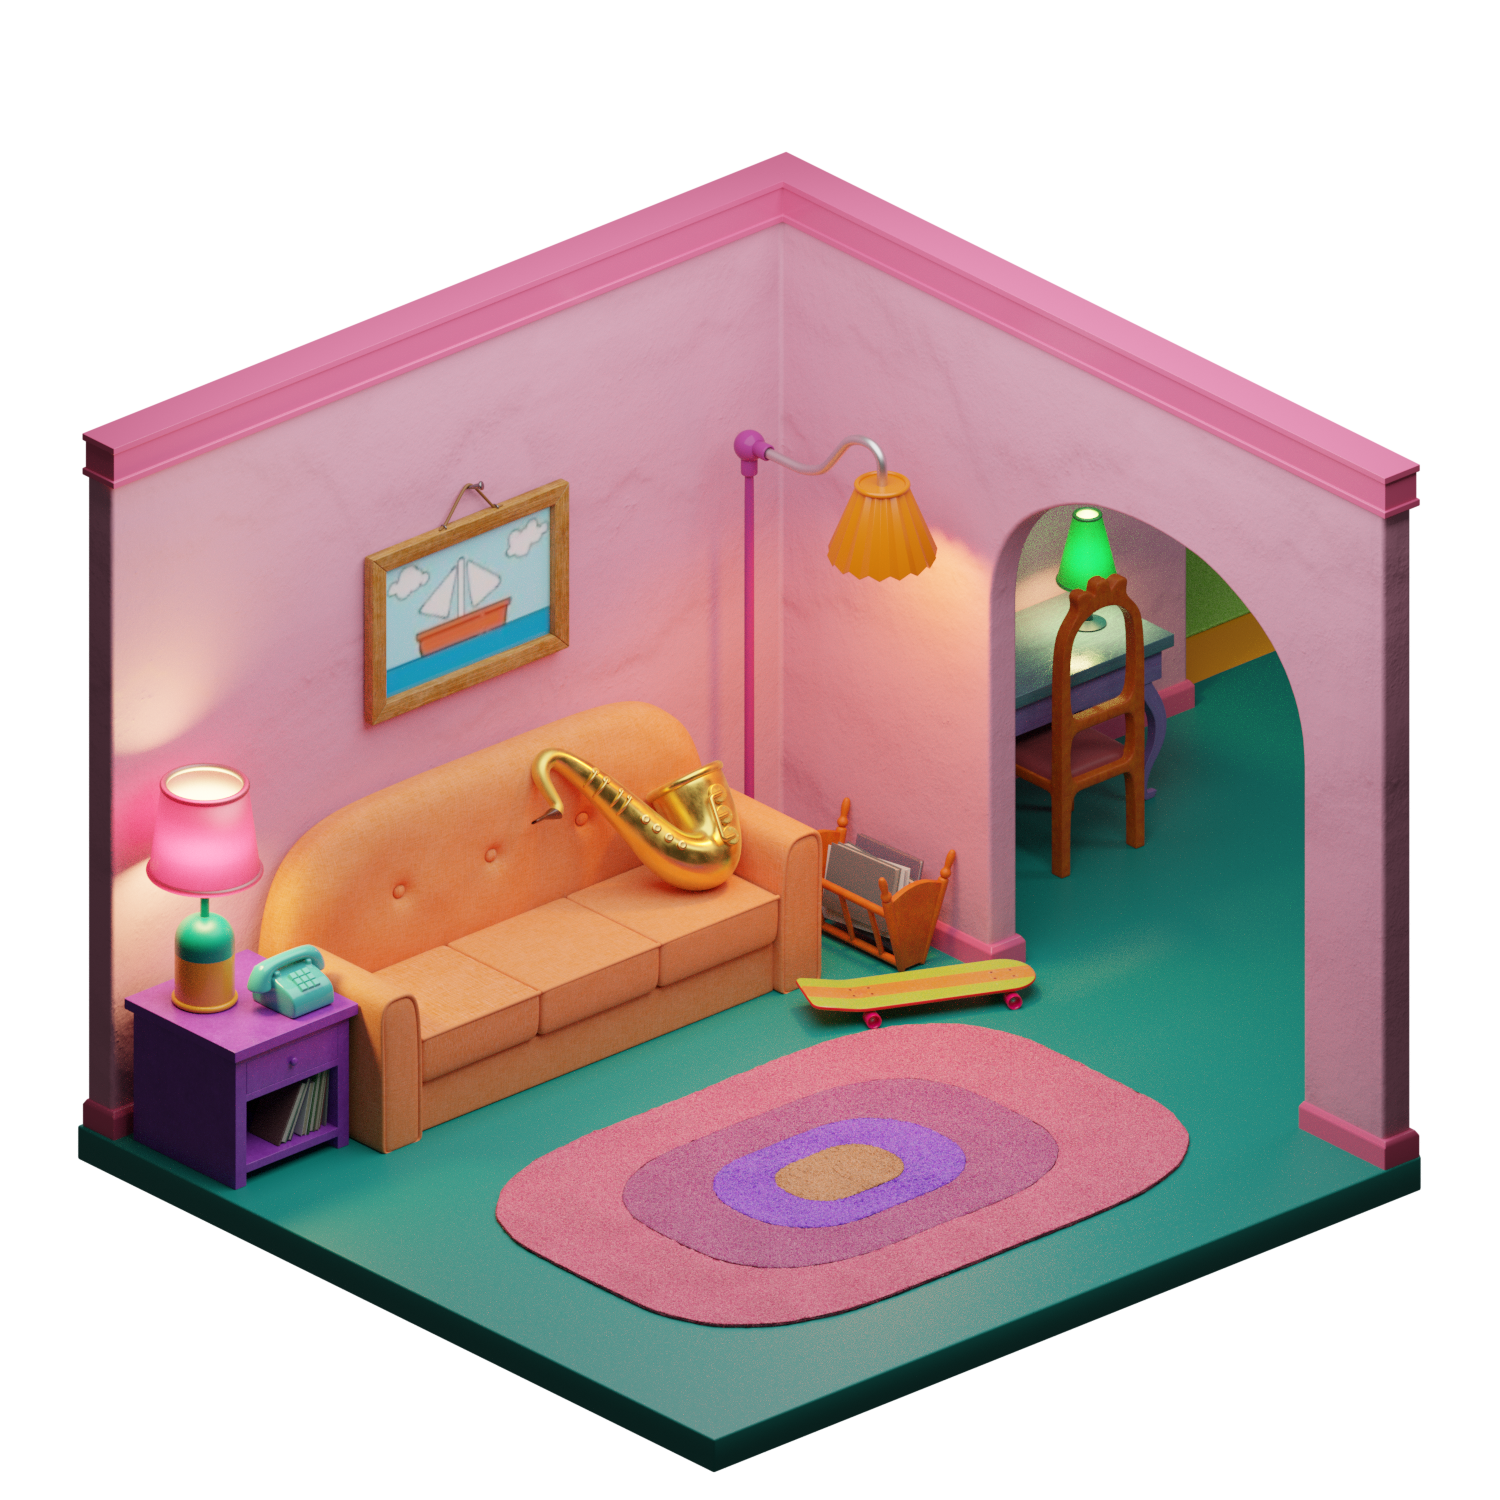
\includegraphics[width=1\linewidth,height=\textheight,keepaspectratio]{../resources/practica9/images/full.png}

\subcaption{\label{}Iluminación completa: \texttt{ka\ +\ kd\ +\ ks}.}
\end{minipage}%
%
\begin{minipage}{0.50\linewidth}

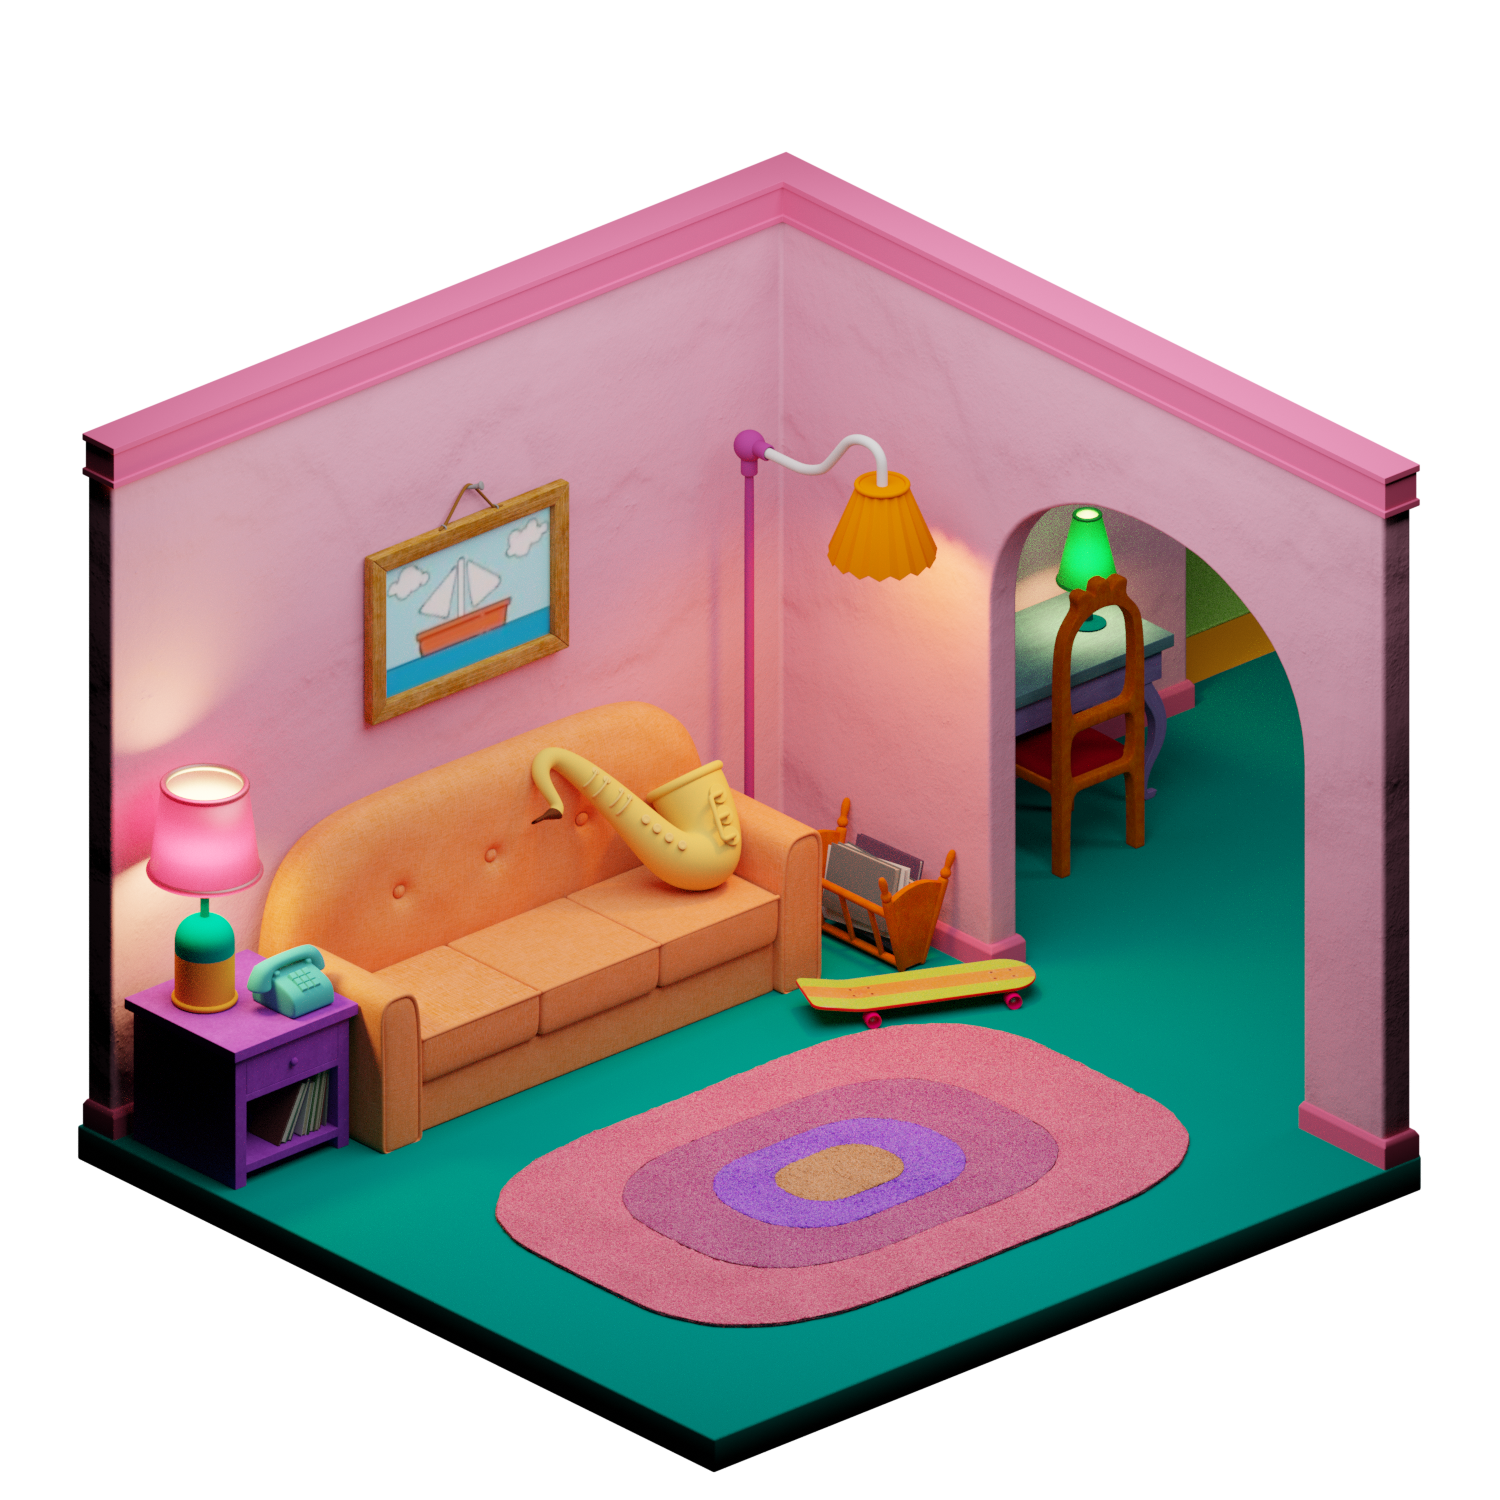
\includegraphics[width=1\linewidth,height=\textheight,keepaspectratio]{../resources/practica9/images/ka_kd.png}

\subcaption{\label{}Sin componente especular: \texttt{ka\ +\ kd}.}
\end{minipage}%

\caption{\label{fig-practica9-phong-specular}Comparación entre el modelo completo y el mismo caso sin componente especular. El brillo más evidente desaparece al quitar \texttt{ks}.}

\end{figure}%

\begin{figure}

\begin{minipage}{0.50\linewidth}

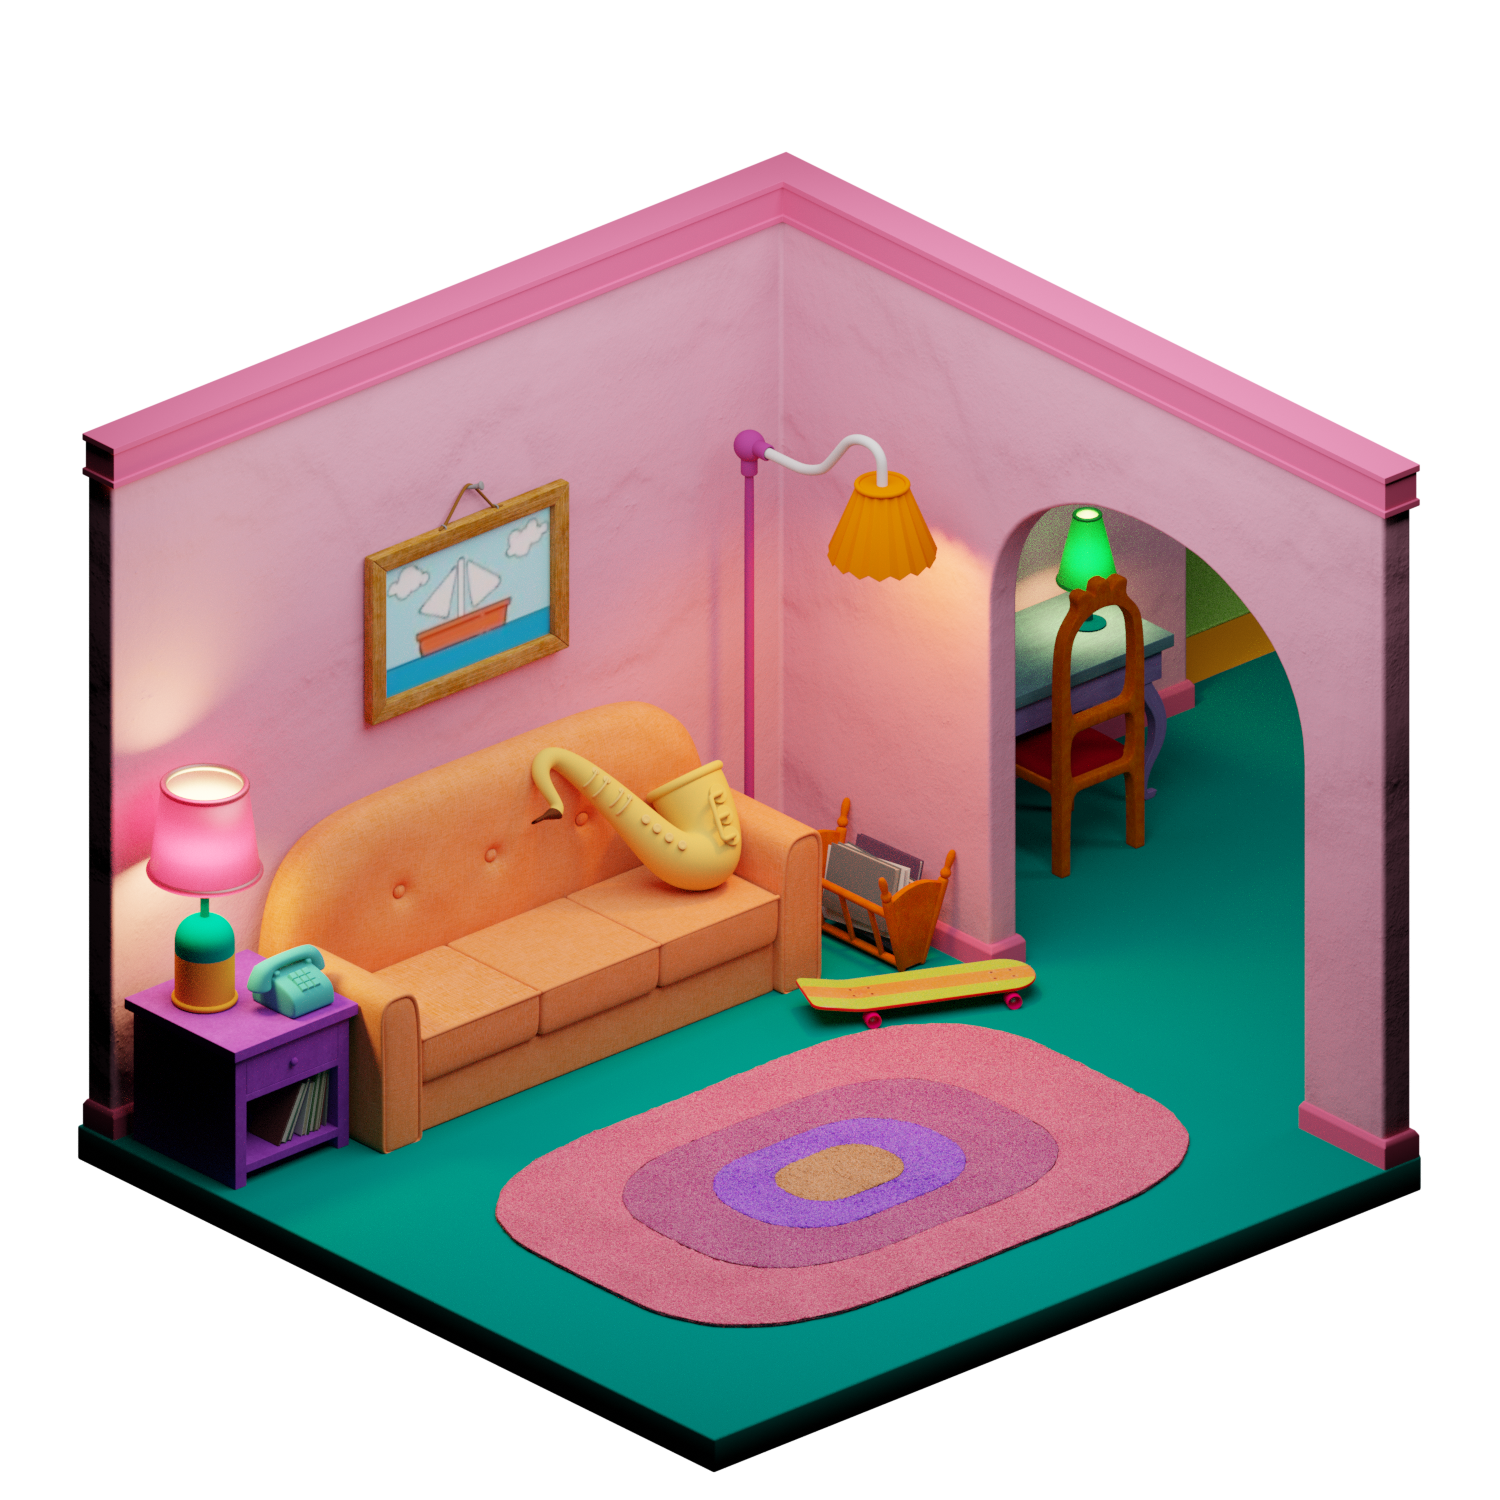
\includegraphics[width=1\linewidth,height=\textheight,keepaspectratio]{../resources/practica9/images/ka_kd.png}

\subcaption{\label{}Ambiente más difusa: \texttt{ka\ +\ kd}.}
\end{minipage}%
%
\begin{minipage}{0.50\linewidth}

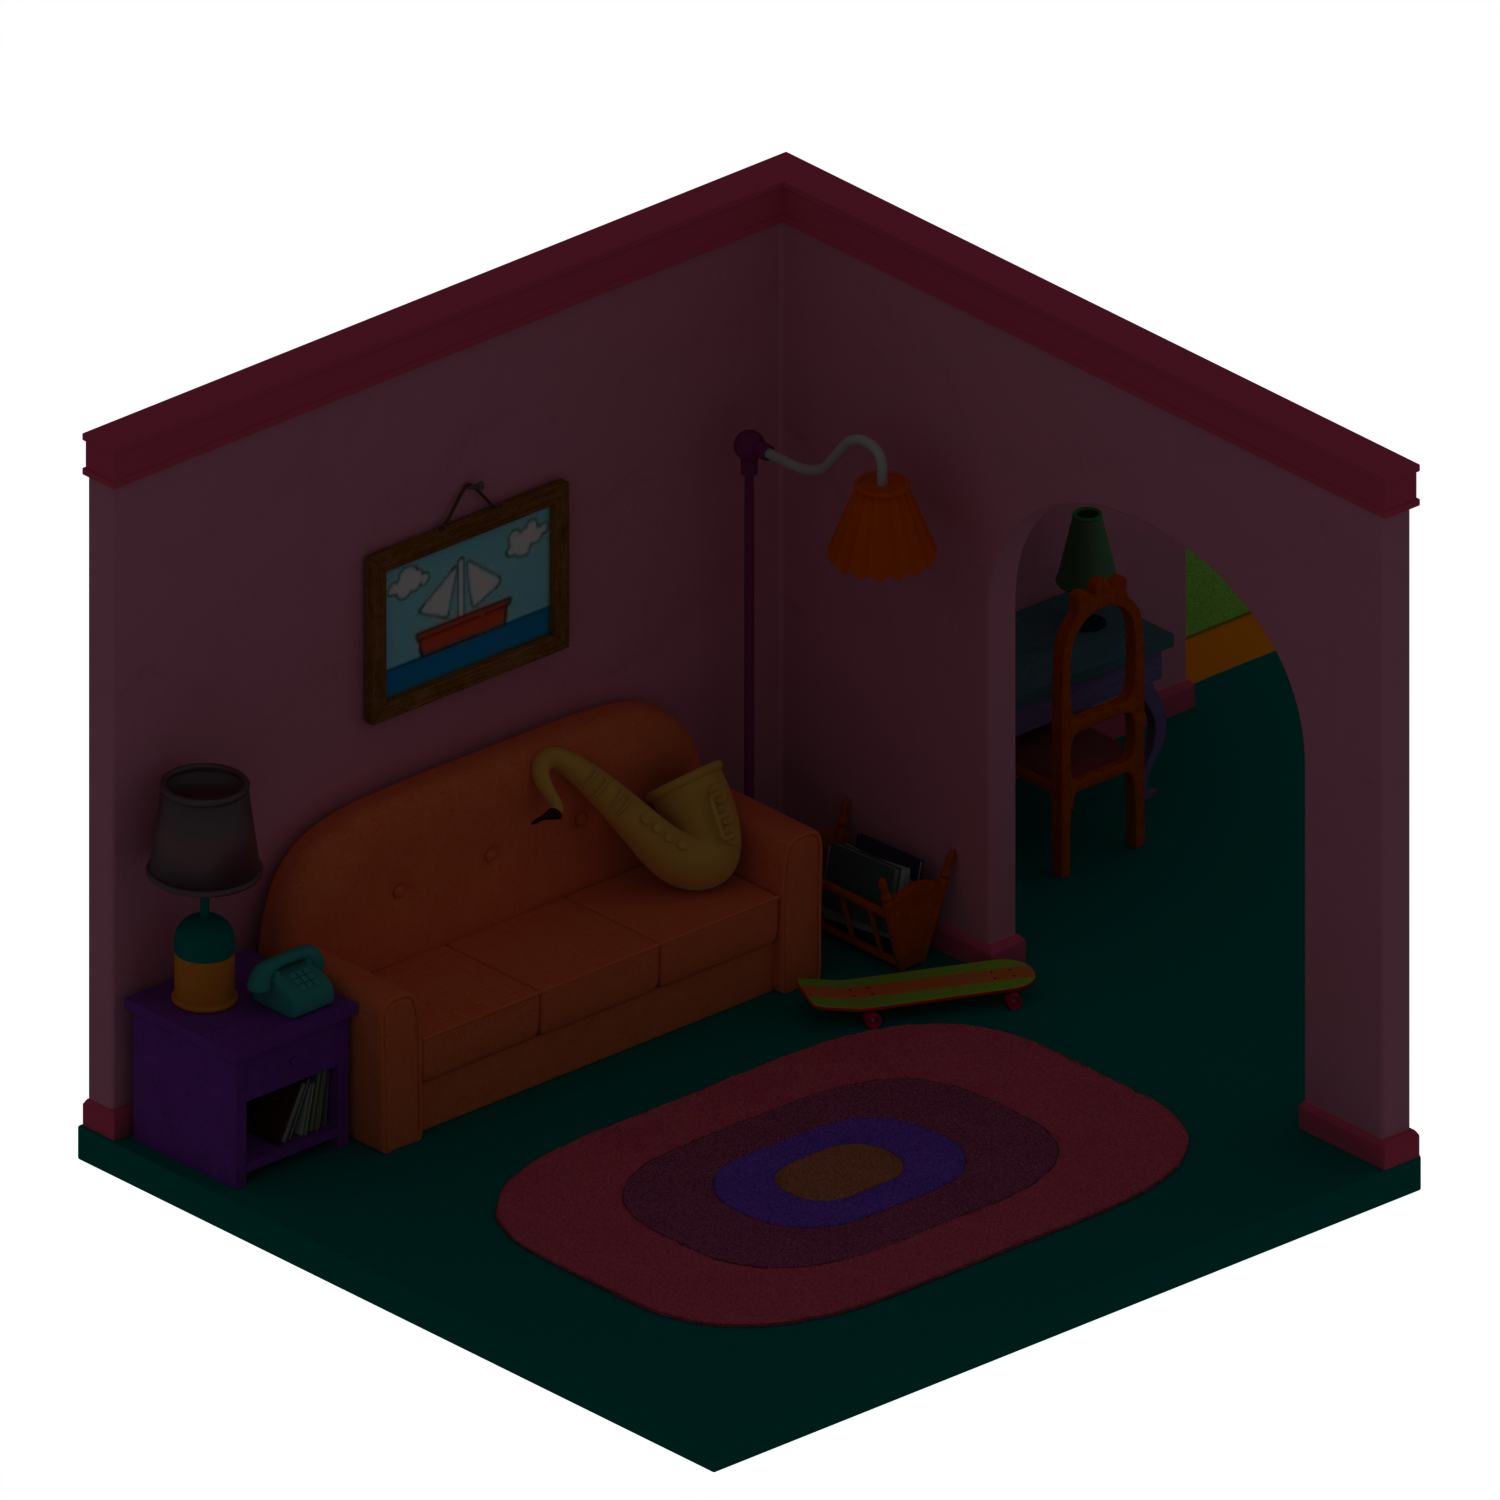
\includegraphics[width=1\linewidth,height=\textheight,keepaspectratio]{../resources/practica9/images/kd.png}

\subcaption{\label{}Solo difusa: \texttt{kd}.}
\end{minipage}%

\caption{\label{fig-practica9-phong-ambient}Comparación entre ambiente más difusa y solo difusa. Sin \texttt{ka}, las zonas menos iluminadas quedan mucho más oscuras. Fuente: escena de BlenderKit, autor: Russo 3D.}

\end{figure}%

\begin{tcolorbox}[enhanced jigsaw, colframe=quarto-callout-note-color-frame, arc=.35mm, bottomrule=.15mm, left=2mm, breakable, opacityback=0, coltitle=black, bottomtitle=1mm, toptitle=1mm, titlerule=0mm, toprule=.15mm, rightrule=.15mm, title={Experimenta con colores}, colbacktitle=quarto-callout-note-color!10!white, opacitybacktitle=0.6, colback=white, leftrule=.75mm]

\begin{itemize}
\item
  Pon en el visualizador una \textbf{luz completamente roja} (canales verde y azul a 0) y el \textbf{material completamente verde} (canales rojo y azul a 0). ¿De qué color queda el objeto? ¿Por qué?
\item
  Prueba con otras combinaciones de colores de luz y material.
\end{itemize}

\end{tcolorbox}

Para responder en PDF, usa la multiplicación por canales. Si la luz es roja pura y el material es verde puro:

\begin{longtable}[]{@{}lrrr@{}}
\toprule\noalign{}
Canal & Luz & Material & Resultado \\
\midrule\noalign{}
\endhead
\bottomrule\noalign{}
\endlastfoot
R & 1.00 & 0.00 & 0.00 \\
G & 0.00 & 1.00 & 0.00 \\
B & 0.00 & 0.00 & 0.00 \\
\end{longtable}

El resultado ambiente/difuso es negro, porque ningún canal coincide entre la luz y el material. Si aparecen brillos especulares, tenderán a seguir el color de la luz.

\begin{tcolorbox}[enhanced jigsaw, colframe=quarto-callout-note-color-frame, arc=.35mm, bottomrule=.15mm, left=2mm, breakable, opacityback=0, coltitle=black, bottomtitle=1mm, toptitle=1mm, titlerule=0mm, toprule=.15mm, rightrule=.15mm, title={Reto de visualización: modo ondas}, colbacktitle=quarto-callout-note-color!10!white, opacitybacktitle=0.6, colback=white, leftrule=.75mm]

Vamos a crear un modo nuevo de visualización, como si el modelo fuese un falso análisis de ondas de color.

Primero, abre \texttt{renderer.RenderMode} y añade un valor nuevo al \texttt{enum}:

\PracticeCode{../resources/practica9/snippets/render-mode-ondas.java}

Después, abre \texttt{renderer.Shader}. Justo después del bloque de \texttt{RenderMode.NORMALS}, añade este caso:

\PracticeCode{../resources/practica9/snippets/shader-render-mode-ondas.java}

Por último, añade este método cerca de \texttt{shadeNormals}. Esta versión ya funciona y suele dar un resultado vistoso:

\PracticeCode{../resources/practica9/snippets/shade-ondas.java}

Dentro de las funciones seno y coseno, puedes combinar las tres ondas de la forma que quieras. Prueba a sumarlas, multiplicarlas o a usarlas por separado, o súmale algún término como \texttt{nx}, \texttt{ny} o \texttt{nz} para que la orientación de la superficie también influya en el resultado. Un posible resultado es este:

\begin{figure}[H]

{\centering \pandocbounded{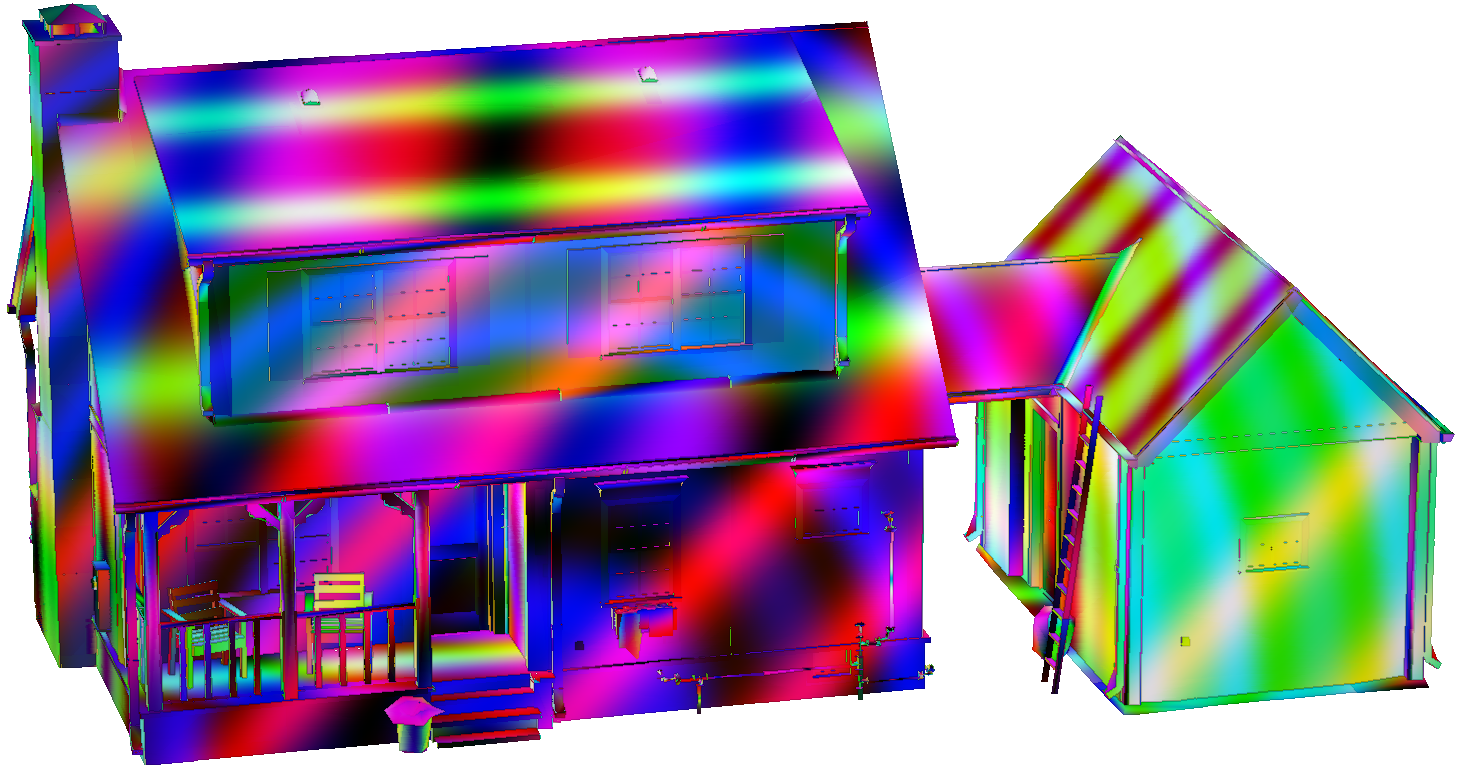
\includegraphics[keepaspectratio]{../resources/practica9/images/render_tan.png}}

}

\caption{Ejemplo de renderizado con nuestro modo ondas.}

\end{figure}%

\end{tcolorbox}

\section{Más allá de Phong}

\label{más-allá-de-phong}

El visualizador de esta práctica no implementa renderizado basado en físicas, y tampoco es el objetivo que lo haga. Aun así, conviene saber que en herramientas profesionales como \textbf{\emph{Blender}} el resultado final suele apoyarse en modelos de iluminación más completos que Phong.

En lugar de decidir el color de un punto solo con la luz directa y un brillo aproximado, estos motores intentan estimar cómo viaja la luz por toda la escena: qué parte llega directamente, qué parte rebota en paredes, suelos, techos o vidrios, y cómo responden los materiales. En arquitectura esto importa mucho, porque la percepción de un espacio depende en gran medida de esos rebotes de luz.

\begin{tcolorbox}[enhanced jigsaw, colframe=quarto-callout-note-color-frame, arc=.35mm, bottomrule=.15mm, left=2mm, breakable, opacityback=0, coltitle=black, bottomtitle=1mm, toptitle=1mm, titlerule=0mm, toprule=.15mm, rightrule=.15mm, title={Qué debes retener}, colbacktitle=quarto-callout-note-color!10!white, opacitybacktitle=0.6, colback=white, leftrule=.75mm]

No necesitas aprender ni programar \textbf{\emph{path tracing}} en esta práctica. Esta sección solo sirve para que, cuando en \emph{Blender} veas palabras como \emph{samples}, \emph{bounces}, \emph{noise} o \emph{Cycles}, sepas a qué se refieren.

\end{tcolorbox}

\begin{tcolorbox}[enhanced jigsaw, colframe=quarto-callout-tip-color-frame, arc=.35mm, bottomrule=.15mm, left=2mm, breakable, opacityback=0, coltitle=black, bottomtitle=1mm, toptitle=1mm, titlerule=0mm, toprule=.15mm, rightrule=.15mm, title={Detalle técnico opcional}, colbacktitle=quarto-callout-tip-color!10!white, opacitybacktitle=0.6, colback=white, leftrule=.75mm]

Si quieres ver la formulación clásica, la idea se resume en la \textbf{ecuación de renderizado} de Kajiya (1986):

\[
L_o(\mathbf{p},\,\omega_o) = L_e(\mathbf{p},\,\omega_o) + \int_{\Omega} f_r(\mathbf{p},\,\omega_o,\,\omega_i)\; L_i(\mathbf{p},\,\omega_i)\; |\cos\theta_i|\; d\omega_i
\]

Sin entrar en todos los símbolos, viene a decir que el color que vemos en un punto depende de la luz que emite ese punto y de toda la luz que le llega después de interactuar con la escena.

\end{tcolorbox}

El esquema interactivo de la versión HTML permite cambiar el número de rayos y el máximo de rebotes. En PDF, la idea se resume así:

\begin{longtable}[]{@{}
  >{\raggedright\arraybackslash}p{(\linewidth - 2\tabcolsep) * \real{0.5000}}
  >{\raggedright\arraybackslash}p{(\linewidth - 2\tabcolsep) * \real{0.5000}}@{}}
\toprule\noalign{}
\begin{minipage}[b]{\linewidth}\raggedright
Elemento
\end{minipage} & \begin{minipage}[b]{\linewidth}\raggedright
Lectura
\end{minipage} \\
\midrule\noalign{}
\endhead
\bottomrule\noalign{}
\endlastfoot
Rayo primario & Sale de la cámara y busca una superficie visible. \\
Rebote & Al chocar con una superficie, nace una nueva dirección aleatoria. \\
Camino que llega a la luz & Aporta energía al píxel. \\
Camino que no llega a la luz & Aporta poca o ninguna energía en esa muestra. \\
\end{longtable}

Al aumentar el número de rayos o la profundidad máxima, crecen las probabilidades de estimar mejor la iluminación indirecta, pero también aumenta el coste de cálculo.

\subsection{Muestras, ruido y convergencia}

\label{muestras-ruido-y-convergencia}

La idea práctica es aproximar esos rebotes con muchas muestras. Si has visto que en \emph{Blender} aparecen parámetros como \texttt{samples} o \texttt{spp} (\emph{samples per pixel}), vienen de aquí: el motor lanza muchas trayectorias posibles de la luz y promedia su resultado.

No hace falta que estudies el método en detalle para esta práctica. Quédate con dos consecuencias muy útiles: con pocas muestras aparece ruido; con muchas, la imagen se estabiliza, pero el tiempo de cálculo aumenta.

La intuición estadística puede verse con un ejemplo muy sencillo: estimar el \textbf{área de un círculo de radio 1} generando puntos aleatorios en el cuadrado \([-1,1]^2\).

\[
\pi \approx 4 \cdot \frac{\text{puntos dentro del círculo}}{\text{puntos totales}}
\]

Con pocas muestras, la estimación fluctúa mucho; con muchas muestras, converge lentamente hacia \(\pi\). Esa es la misma intuición que se usa al aumentar las muestras por píxel en un render.

En el renderizado ocurre lo mismo: desde cada píxel se lanzan rayos aleatorios que rebotan entre superficies. Con \textbf{pocas muestras por píxel} (\emph{spp}) el resultado es muy ruidoso; con \textbf{muchas muestras la imagen se va estabilizando}.

\PracticeImagePair
  {fig-practica9-spp}
  {Comparación de convergencia en Blender Cycles: 50 spp frente a 500 spp. \PracticeCredit{Fuente: escena procedente de BlenderKit, autor: Ibrohim Toxirov.}}
  {../resources/practica9/images/room_50spp.png}
  {50 spp: resultado ruidoso, unos 3 min.}
  {../resources/practica9/images/room_500spp.png}
  {500 spp: resultado estable, unos 8 min.}

Esto es lo que ocurre en \emph{Blender Cycles} y en otros motores con visualización realista: con pocas muestras aparece ruido, mientras que con más muestras el resultado se limpia, aunque el tiempo de cálculo también aumenta. En visualización de edificios se puede utilizar para reproducir mucho mejor la iluminación global de interiores y exteriores.

Para esta práctica, sin embargo, lo importante es que nuestro visualizador no busca ese nivel de realismo, sino \emph{una respuesta rápida e interactiva}. Por eso usamos Phong.




\end{document}
